% !TeX program = xelatex
\documentclass[a4paper,10pt]{article}

% ============================================================================
% កញ្ចប់សម្ភារៈសិក្សាបោះពុម្ព ស-ខ្មៅ (Printable Classroom Materials - Grade 8 2.3 POW23)
% មេរៀនទី២៖ ស្វ័យគុណ — ២.៣. វិធីចែកស្វ័យគុណមាននិទស្សន្តរ៉ឺឡាទីប
% ត្រូវគ្នា ១០០% នឹង Research_Brief_POW23.md, LS_Plan_POW23.tex, Teaching_Scenario_POW23.tex
% ============================================================================
\usepackage[a4paper, left=1.0cm, right=1.0cm, top=0.75cm, bottom=1.05cm, footskip=0.55cm]{geometry}
\usepackage{amsmath, amssymb}
\usepackage{unicode-math}
\usepackage{fontspec}
\usepackage{array, colortbl}
\usepackage[table]{xcolor}
\usepackage{enumitem}
\usepackage{pifont}
\usepackage{fancyhdr}
\usepackage{lastpage}
\usepackage{tikz}
\usepackage[most]{tcolorbox}
\usetikzlibrary{calc, arrows.meta, patterns, decorations.markings, decorations.pathreplacing, positioning, babel}

% LaTeX 2025 compatibility guard
\makeatletter
\let\@expl@@@mark@update@singlecol@structures@@\relax
\makeatother

% ============================================================================
% ការកំណត់ពុម្ពអក្សរផ្លូវការ (Cross-Platform Windows + Linux/Cloud fonts/)
% ============================================================================
\providecommand{\NGSFindFonts}{%
  \IfFileExists{C:/Windows/Fonts/cambria.ttc}{%
    \def\NGSSysPath{C:/Windows/Fonts/}%
    \def\NGSUserPath{C:/Users/KIT/AppData/Local/Microsoft/Windows/Fonts/}%
  }{%
    \IfFileExists{./fonts/KhmerOSsiemreap.ttf}{\def\NGSSysPath{./fonts/}\def\NGSUserPath{./fonts/}}{%
    \IfFileExists{../fonts/KhmerOSsiemreap.ttf}{\def\NGSSysPath{../fonts/}\def\NGSUserPath{../fonts/}}{%
    \IfFileExists{../../fonts/KhmerOSsiemreap.ttf}{\def\NGSSysPath{../../fonts/}\def\NGSUserPath{../../fonts/}}{%
    \IfFileExists{../../../fonts/KhmerOSsiemreap.ttf}{\def\NGSSysPath{../../../fonts/}\def\NGSUserPath{../../../fonts/}}{%
    \IfFileExists{../../../../fonts/KhmerOSsiemreap.ttf}{\def\NGSSysPath{../../../../fonts/}\def\NGSUserPath{../../../../fonts/}}{%
    \IfFileExists{../../../../../fonts/KhmerOSsiemreap.ttf}{\def\NGSSysPath{../../../../../fonts/}\def\NGSUserPath{../../../../../fonts/}}{%
    \IfFileExists{../../../../../../fonts/KhmerOSsiemreap.ttf}{\def\NGSSysPath{../../../../../../fonts/}\def\NGSUserPath{../../../../../../fonts/}}{%
      \def\NGSSysPath{../../../../../../../fonts/}\def\NGSUserPath{../../../../../../../fonts/}%
    }}}}}}}%
  }%
}
\NGSFindFonts

\setmathfont[
  Path={\NGSSysPath},
  FontIndex=1,
  Scale=1.02
]{cambria.ttc}

\defaultfontfeatures{Ligatures=TeX}

\setmainfont[
  Path={\NGSUserPath},
  Extension=.ttf,
  Script=Khmer,
  BoldFont={KhmerOSsiemreap},
  BoldFeatures={FakeBold=1.8},
  ItalicFont={KhmerOSsiemreap},
  ItalicFeatures={FakeSlant=0.25},
  BoldItalicFont={KhmerOSsiemreap},
  BoldItalicFeatures={FakeBold=1.8, FakeSlant=0.25}
]{KhmerOSsiemreap}

\newfontfamily\muol[
  Path={\NGSUserPath},
  Extension=.ttf,
  Script=Khmer
]{KhmerOSmuollight}

\newfontfamily\TimesEn[
  Path={\NGSSysPath},
  Extension=.ttf,
  BoldFont={timesbd},
  ItalicFont={timesi},
  BoldItalicFont={timesbi}
]{times}

\newfontfamily\CalibriFont[
  Path={\NGSSysPath},
  Extension=.ttf
]{calibri}

\newfontfamily\Tacteing[
  Path={\NGSUserPath}
]{TACTENG.TTF}

\XeTeXlinebreaklocale "km"
\XeTeXlinebreakskip = 0pt plus 1pt minus 0.1pt

% ============================================================================
% ក្ដារពណ៌ ស-ខ្មៅ សុទ្ធសម្រាប់ការបោះពុម្ព (Strict Monochrome Print Palette)
% ============================================================================
\definecolor{panelgray}{gray}{0.92} % ~gray!8
\definecolor{headgray}{gray}{0.85}  % ~gray!15
\definecolor{midgray}{gray}{0.75}   % ~gray!25
\definecolor{darkline}{gray}{0.35}  % ~gray!65

\pagestyle{fancy}
\fancyhf{}
\renewcommand{\headrulewidth}{0pt}
\fancyfoot[L]{\fontsize{7.6pt}{10pt}\selectfont អនុវិទ្យាល័យព្រះក្រសាំង \en{---} គណិតវិទ្យា ថ្នាក់ទី៨ \en{|} មេរៀនទី២ (២.៣) វិធីចែកស្វ័យគុណ (ស-ខ្មៅ) \en{|} ថ្ងៃចន្ទ ៧កើត កត្តិក ២៥៧០ \en{|} ១៦ វិច្ឆិកា ២០២៦}
\fancyfoot[R]{\fontsize{8.2pt}{10pt}\selectfont ទំព័រ \en{\thepage\ / \pageref{LastPage}}}

\setlength{\parindent}{0pt}
\setlength{\parskip}{0pt}
\setlength{\tabcolsep}{4pt}

% ============================================================================
% ម៉ាក្រូជំនួយ (Helper Macros)
% ============================================================================
\newcommand{\en}[1]{{\TimesEn #1}}
\newcommand{\enbf}[1]{{\TimesEn\bfseries #1}}
\newcommand{\unit}[1]{\,\text{\en{#1}}}
\newcommand{\cnum}[1]{\mbox{\fontsize{10pt}{12pt}\selectfont\ding{\numexpr181+#1\relax}}}
\newcommand{\blankcnum}{\tikz[baseline=-0.65ex]\draw[black, line width=0.8pt] (0,0) circle (0.16cm);}
\newcommand{\scissors}{\ding{34}}
\newcommand{\chkbox}{\tikz[baseline=-0.15ex]\draw[black, line width=0.85pt] (0,0) rectangle (0.24cm,0.24cm);}
\newcommand{\stk}[1]{\tikz[baseline=(n.base)]{\node[inner sep=0.6pt](n){$#1$}; \draw[black, line width=0.85pt] (n.south west)--(n.north east);}}
\newcommand{\khmflourish}{{\Tacteing\fontsize{32pt}{13pt}\selectfont\raisebox{-4pt}{3}}}

\newcommand{\pagebanner}[2]{%
  \begin{tcolorbox}[
    enhanced, sharp corners, colback=headgray, colframe=black,
    boxrule=1.1pt, boxsep=1pt, top=3pt, bottom=3pt, left=6pt, right=6pt,
    after skip=4pt
  ]
    {\muol\fontsize{9.0pt}{13.5pt}\selectfont #1}\hfill{\fontsize{8.0pt}{11.5pt}\selectfont\textbf{#2}}
  \end{tcolorbox}%
}

\newcolumntype{L}[1]{>{\raggedright\arraybackslash}p{#1}}
\newcolumntype{C}[1]{>{\centering\arraybackslash}p{#1}}

\begin{document}
\fontsize{9.0pt}{13.2pt}\selectfont

% ============================================================================
% ទំព័រទី ១៖ សម្ភារៈ E2 សកម្មភាព 1 ខ្នាតពិត 1:1 (បន្ទះកាត់ 2^7/2^4 និង 3^7/3^5)
% ============================================================================
\pagebanner{សម្ភារៈទី ១៖ បន្ទះកាត់ \enbf{E2} សកម្មភាព \enbf{1} ខ្នាតពិត \enbf{1:1 --} កាត់កត្តារួម \enbf{2\textsuperscript{7}}$\div$\enbf{2\textsuperscript{4}} និង \enbf{3\textsuperscript{7}}$\div$\enbf{3\textsuperscript{5}}}{ទំព័រ ១/៦ \en{-- E2 Act 1}}

% --- ប្រអប់ព្រមានខ្នាតពិត & បន្ទះផ្ទៀង 5.00 cm (x=1cm, y=1cm) ---
\noindent
\begin{minipage}[c]{11.9cm}
  \begin{tcolorbox}[
    enhanced, sharp corners, colback=panelgray, colframe=black,
    boxrule=1.0pt, boxsep=1pt, top=3pt, bottom=3pt, left=6pt, right=6pt
  ]
    \fontsize{8.0pt}{11.4pt}\selectfont
    \textbf{ការណែនាំបោះពុម្ពខ្នាតពិត (\en{Print at 100\% / Actual Size})៖} ជ្រើស \textbf{\en{Scale: Actual Size 100\%}} \en{--} \textbf{ហាម \en{Fit to Page}} ដើម្បីឱ្យប្រវែងប្រអប់កត្តានីមួយៗស្មើ \textbf{\en{1.00 cm}} ពិត ($7\text{ កត្តា} = 7.00\unit{cm}$, $4\text{ កត្តា} = 4.00\unit{cm}$, $5\text{ កត្តា} = 5.00\unit{cm}$)។\\[2pt]
    \textbf{ក្រុមវិស្វករទិន្នន័យកុំព្យូទ័រ (\en{E2 Act 1})៖} កាត់ \scissors{} បន្ទះភាគយក និងភាគបែង រួចផ្ទឹមតម្រៀប ១-ទល់-១ ហើយគូសឈូស \en{/} កត្តាដូចគ្នា ($\frac{a}{a}=1$) ដើម្បីរកកត្តាសល់!
  \end{tcolorbox}
\end{minipage}%
\hfill
\begin{minipage}[c]{6.8cm}
  \begin{tcolorbox}[
    enhanced, sharp corners, colback=white, colframe=black,
    boxrule=1.0pt, boxsep=1pt, top=2.5pt, bottom=2.5pt, left=4pt, right=4pt
  ]
    \centering
    {\fontsize{7.7pt}{9.8pt}\selectfont\textbf{បន្ទះផ្ទៀងខ្នាតពិត \en{5.00 cm} (\en{Actual Size 100\%})}}\\[1.5pt]
    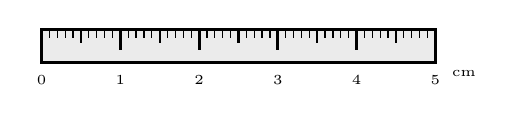
\begin{tikzpicture}[x=1cm, y=1cm, every node/.style={font=\scriptsize, text=black}]
      \draw[black, line width=1.1pt, fill=panelgray] (0,0) rectangle (5.0, 0.42);
      \foreach \m in {0,...,50}{
        \pgfmathsetmacro{\xval}{\m*0.1}
        \draw[black, line width=0.45pt] (\xval, 0.42) -- (\xval, 0.31);
      }
      \foreach \h in {0,0.5,...,5.0}{
        \draw[black, line width=0.8pt] (\h, 0.42) -- (\h, 0.24);
      }
      \foreach \c in {0,1,2,3,4,5}{
        \draw[black, line width=1.1pt] (\c, 0.42) -- (\c, 0.15);
        \node[below=1pt, font=\tiny] at (\c, 0.0) {\en{\c}};
      }
      \node[right=2pt, font=\tiny] at (5.02, -0.14) {\en{cm}};
    \end{tikzpicture}
  \end{tcolorbox}
\end{minipage}

\vspace{5pt}

\begin{tcolorbox}[
  enhanced, sharp corners, colback=white, colframe=black,
  boxrule=0.8pt, boxsep=1pt, top=3pt, bottom=3pt, left=6pt, right=6pt, after skip=6pt
]
  \fontsize{7.8pt}{10.8pt}\selectfont
  \textbf{ក្រុម៖} $\underline{\hspace{1.2cm}}$ \quad \textbf{សមាជិក ៣ នាក់៖} ១. $\underline{\hspace{2.9cm}}$ \quad ២. $\underline{\hspace{2.9cm}}$ \quad ៣. $\underline{\hspace{2.9cm}}$ \quad \textbf{កាលបរិច្ឆេទ៖} \en{16/11/2026}
\end{tcolorbox}

% --- ផ្នែកទី ១៖ កញ្ចប់ A (ឧទាហរណ៍ ក — ទំព័រ ១៦, កែតម្រូវពេញ ៧ កត្តា!) ---
\textbf{១. កញ្ចប់ \en{A} (ឧទាហរណ៍ ក \en{--} ទំ.១៦)៖ $\dfrac{2^7}{2^4}$} \quad {\fontsize{8.1pt}{11pt}\selectfont\textit{(កែតម្រូវសៀវភៅទំ.១៦ ដែលបោះពុម្ពខ្វះ ៦ កត្តា $\to$ ទីនេះបោះពុម្ព \textbf{៧ កត្តាពេញ}!)}}

\vspace{3pt}
\noindent
\begin{minipage}[c]{9.75cm}
  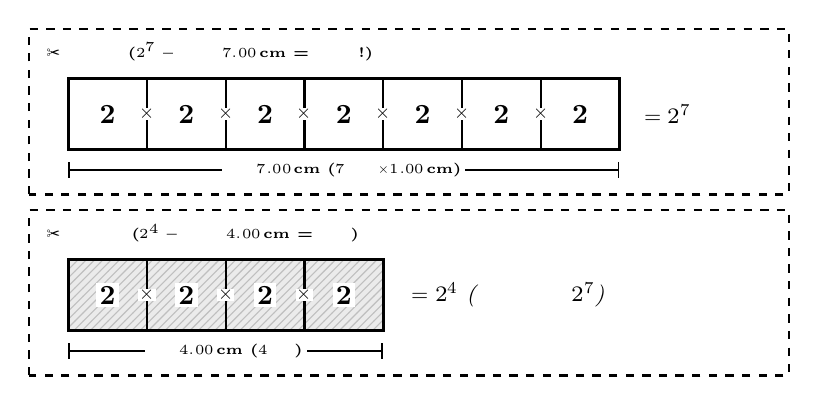
\begin{tikzpicture}[x=1cm, y=1cm, every node/.style={font=\footnotesize, text=black}]
    % Cuttable Numerator Strip: 2^7 = 7 factors * 1.00 cm = 7.00 cm
    \draw[black, dashed, line width=0.9pt] (0, 2.35) rectangle (9.65, 4.45);
    \node[anchor=north west, font=\tiny] at (0.10, 4.40) {\scissors\ \textbf{កាត់បន្ទះភាគយក ($2^7$ \en{--} ប្រវែងពិត $7.00\unit{cm}$ = ៧ កត្តាពេញ!)}};

    \fill[white] (0.50, 2.92) rectangle (7.50, 3.82);
    \draw[black, line width=1.2pt] (0.50, 2.92) rectangle (7.50, 3.82);
    \foreach \i in {1,...,6}{
      \draw[black, line width=0.85pt] (0.50+\i, 2.92) -- (0.50+\i, 3.82);
      \node[fill=white, inner sep=0.5pt, font=\scriptsize] at (0.50+\i, 3.37) {$\times$};
    }
    \foreach \i in {0,...,6}{
      \node[font=\normalsize] at (1.00+\i, 3.37) {$\mathbf{2}$};
    }
    \node[right=4pt, font=\footnotesize] at (7.55, 3.37) {$= 2^7$};
    \draw[black, line width=0.7pt, {Bar[width=2mm]}-{Bar[width=2mm]}] (0.50, 2.66) -- (7.50, 2.66);
    \node[fill=white, inner sep=1.5pt, font=\tiny] at (4.00, 2.66) {\textbf{ប្រវែង $7.00\unit{cm}$ ($7$ កត្តា $\times 1.00\unit{cm}$)}};

    % Cuttable Denominator Strip: 2^4 = 4 factors * 1.00 cm = 4.00 cm
    \draw[black, dashed, line width=0.9pt] (0, 0.05) rectangle (9.65, 2.15);
    \node[anchor=north west, font=\tiny] at (0.10, 2.10) {\scissors\ \textbf{កាត់បន្ទះភាគបែង ($2^4$ \en{--} ប្រវែងពិត $4.00\unit{cm}$ = ៤ កត្តា)}};

    \fill[panelgray] (0.50, 0.62) rectangle (4.50, 1.52);
    \pattern[pattern=north east lines, pattern color=midgray] (0.50, 0.62) rectangle (4.50, 1.52);
    \draw[black, line width=1.2pt] (0.50, 0.62) rectangle (4.50, 1.52);
    \foreach \i in {1,...,3}{
      \draw[black, line width=0.85pt] (0.50+\i, 0.62) -- (0.50+\i, 1.52);
      \node[fill=white, inner sep=0.4pt, font=\scriptsize] at (0.50+\i, 1.07) {$\times$};
    }
    \foreach \i in {0,...,3}{
      \node[fill=white, inner sep=1.2pt, font=\normalsize] at (1.00+\i, 1.07) {$\mathbf{2}$};
    }
    \node[right=4pt, font=\footnotesize] at (4.60, 1.07) {$= 2^4$ \textit{(ដាក់ផ្ទឹមក្រោម $2^7$)}};
    \draw[black, line width=0.7pt, {Bar[width=2mm]}-{Bar[width=2mm]}] (0.50, 0.36) -- (4.50, 0.36);
    \node[fill=white, inner sep=1.5pt, font=\tiny] at (2.50, 0.36) {\textbf{ប្រវែង $4.00\unit{cm}$ ($4$ កត្តា)}};
  \end{tikzpicture}
\end{minipage}%
\hfill
\begin{minipage}[c]{8.95cm}
  \begin{tcolorbox}[
    enhanced, sharp corners, colback=white, colframe=black,
    boxrule=1.0pt, boxsep=1pt, top=4pt, bottom=4pt, left=5.5pt, right=5.5pt,
    title={\textbf{កំណត់ត្រាពិសោធន៍ កញ្ចប់ \en{A} ($\dfrac{2^7}{2^4}$)}},
    colbacktitle=headgray, coltitle=black, fonttitle=\fontsize{8.1pt}{11.0pt}\selectfont
  ]
    \raggedright\fontsize{7.8pt}{11.5pt}\selectfont
    \textbf{១. ទស្សន៍ទាយ (\en{E1 Hook})៖} $\dfrac{2^7}{2^4} = \chkbox\,1^3 \quad \chkbox\,2^{\frac{7}{4}} \quad \chkbox\,2^3$\\[3pt]
    \textbf{២. សម្រួលកត្តា ១-ទល់-១ ($\frac{2}{2}=1$)៖}\\
    $\dfrac{2^7}{2^4} = \dfrac{2\times 2\times 2\times 2\times 2\times 2\times 2}{2\times 2\times 2\times 2}$ \quad \textit{(គ្រប់ $7$ កត្តា!)}\\[3pt]
    $\bullet$ គូកត្តា $\frac{2}{2}=1$ ដែលកាត់ចោលមាន $\underline{\hspace{0.55cm}}$ គូ \chkbox\\[3pt]
    $\bullet$ កត្តា $2$ ដែលនៅសល់លើភាគយកមាន $\underline{\hspace{0.55cm}}$ កត្តា \chkbox\\[3pt]
    $\Rightarrow \dfrac{2^7}{2^4} = 2^{\underline{\hspace{0.4cm}}-\underline{\hspace{0.4cm}}} = 2^{\underline{\hspace{0.35cm}}} = \underline{\hspace{0.65cm}}$ \quad \textit{(គោល \textbf{2} នៅដដែល!)}
  \end{tcolorbox}
\end{minipage}

\vspace{10pt}

% --- ផ្នែកទី ២៖ កញ្ចប់ B (ឧទាហរណ៍ ខ — ទំព័រ ១៦: 3^7 / 3^5) ---
\textbf{២. កញ្ចប់ \en{B} (ឧទាហរណ៍ ខ \en{--} ទំ.១៦)៖ $\dfrac{3^7}{3^5}$} \quad {\fontsize{8.1pt}{11pt}\selectfont\textit{(បន្ទះកាត់ ១:១ សម្រាប់គោល $3$ \en{--} ប្រវែង $7.00\unit{cm}$ ធៀបនឹង $5.00\unit{cm}$)}}

\vspace{3pt}
\noindent
\begin{minipage}[c]{9.75cm}
  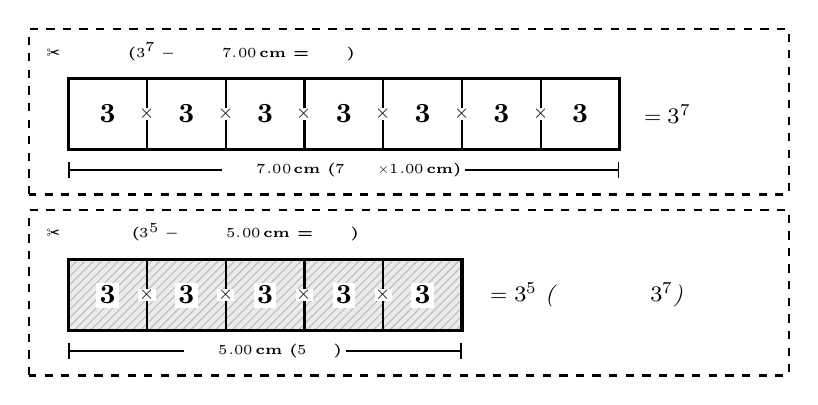
\begin{tikzpicture}[x=1cm, y=1cm, every node/.style={font=\footnotesize, text=black}]
    % Cuttable Numerator Strip: 3^7 = 7 factors * 1.00 cm = 7.00 cm
    \draw[black, dashed, line width=0.9pt] (0, 2.35) rectangle (9.65, 4.45);
    \node[anchor=north west, font=\tiny] at (0.10, 4.40) {\scissors\ \textbf{កាត់បន្ទះភាគយក ($3^7$ \en{--} ប្រវែងពិត $7.00\unit{cm}$ = ៧ កត្តា)}};

    \fill[white] (0.50, 2.92) rectangle (7.50, 3.82);
    \draw[black, line width=1.2pt] (0.50, 2.92) rectangle (7.50, 3.82);
    \foreach \i in {1,...,6}{
      \draw[black, line width=0.85pt] (0.50+\i, 2.92) -- (0.50+\i, 3.82);
      \node[fill=white, inner sep=0.5pt, font=\scriptsize] at (0.50+\i, 3.37) {$\times$};
    }
    \foreach \i in {0,...,6}{
      \node[font=\normalsize] at (1.00+\i, 3.37) {$\mathbf{3}$};
    }
    \node[right=4pt, font=\footnotesize] at (7.55, 3.37) {$= 3^7$};
    \draw[black, line width=0.7pt, {Bar[width=2mm]}-{Bar[width=2mm]}] (0.50, 2.66) -- (7.50, 2.66);
    \node[fill=white, inner sep=1.5pt, font=\tiny] at (4.00, 2.66) {\textbf{ប្រវែង $7.00\unit{cm}$ ($7$ កត្តា $\times 1.00\unit{cm}$)}};

    % Cuttable Denominator Strip: 3^5 = 5 factors * 1.00 cm = 5.00 cm
    \draw[black, dashed, line width=0.9pt] (0, 0.05) rectangle (9.65, 2.15);
    \node[anchor=north west, font=\tiny] at (0.10, 2.10) {\scissors\ \textbf{កាត់បន្ទះភាគបែង ($3^5$ \en{--} ប្រវែងពិត $5.00\unit{cm}$ = ៥ កត្តា)}};

    \fill[panelgray] (0.50, 0.62) rectangle (5.50, 1.52);
    \pattern[pattern=north east lines, pattern color=midgray] (0.50, 0.62) rectangle (5.50, 1.52);
    \draw[black, line width=1.2pt] (0.50, 0.62) rectangle (5.50, 1.52);
    \foreach \i in {1,...,4}{
      \draw[black, line width=0.85pt] (0.50+\i, 0.62) -- (0.50+\i, 1.52);
      \node[fill=white, inner sep=0.4pt, font=\scriptsize] at (0.50+\i, 1.07) {$\times$};
    }
    \foreach \i in {0,...,4}{
      \node[fill=white, inner sep=1.2pt, font=\normalsize] at (1.00+\i, 1.07) {$\mathbf{3}$};
    }
    \node[right=4pt, font=\footnotesize] at (5.60, 1.07) {$= 3^5$ \textit{(ដាក់ផ្ទឹមក្រោម $3^7$)}};
    \draw[black, line width=0.7pt, {Bar[width=2mm]}-{Bar[width=2mm]}] (0.50, 0.36) -- (5.50, 0.36);
    \node[fill=white, inner sep=1.5pt, font=\tiny] at (3.00, 0.36) {\textbf{ប្រវែង $5.00\unit{cm}$ ($5$ កត្តា)}};
  \end{tikzpicture}
\end{minipage}%
\hfill
\begin{minipage}[c]{8.95cm}
  \begin{tcolorbox}[
    enhanced, sharp corners, colback=white, colframe=black,
    boxrule=1.0pt, boxsep=1pt, top=4pt, bottom=4pt, left=5.5pt, right=5.5pt,
    title={\textbf{កំណត់ត្រាពិសោធន៍ កញ្ចប់ \en{B} ($\dfrac{3^7}{3^5}$)}},
    colbacktitle=headgray, coltitle=black, fonttitle=\fontsize{8.1pt}{11.0pt}\selectfont
  ]
    \raggedright\fontsize{7.8pt}{11.5pt}\selectfont
    \textbf{១. តម្រៀបផ្ទឹម ១-ទល់-១ និងកាត់គូរួម ($\frac{3}{3}=1$)៖}\\
    $\dfrac{3^7}{3^5} = \dfrac{3\times 3\times 3\times 3\times 3\times 3\times 3}{3\times 3\times 3\times 3\times 3}$\\[3pt]
    $\bullet$ ចំនួនគូ $\frac{3}{3}=1$ ដែលសម្រួលអស់មាន $\underline{\hspace{0.55cm}}$ គូ \chkbox\\[3pt]
    $\bullet$ ចំនួនកត្តា $3$ នៅសល់លើភាគយកមាន $\underline{\hspace{0.55cm}}$ កត្តា \chkbox\\[3pt]
    $\Rightarrow \dfrac{3^7}{3^5} = 3^{\underline{\hspace{0.4cm}}-\underline{\hspace{0.4cm}}} = 3^{\underline{\hspace{0.35cm}}} = \underline{\hspace{0.65cm}}$\\[3pt]
    \textbf{២. ផ្ទៀងខ្នាតប្រវែង៖} $7.00\unit{cm} - 5.00\unit{cm} = \underline{\hspace{0.7cm}}\unit{cm}$ ($2$ ប្រអប់!)
  \end{tcolorbox}
\end{minipage}

\vspace{10pt}

% --- ផ្នែកទី ៣៖ គំរូសម្គាល់ការកាត់គូ 1-ទល់-1 & សន្និដ្ឋានដំបូង (E2 Act 1 + E1 Hook) ---
\begin{tcolorbox}[
  enhanced, sharp corners, colback=panelgray, colframe=black,
  boxrule=1.05pt, boxsep=1pt, top=7pt, bottom=8pt, left=6.5pt, right=6.5pt,
  title={\textbf{សន្និដ្ឋាន \en{E2} សកម្មភាព \en{1}៖ ទាញរូបមន្តចែកស្វ័យគុណគោលដូចគ្នា ($m > n$, $a\neq 0$) និងផ្ទៀងទិន្នន័យ \en{NGS}}},
  colbacktitle=headgray, coltitle=black, fonttitle=\fontsize{8.3pt}{11.4pt}\selectfont
]
  \noindent
  \begin{minipage}[c]{8.55cm}
    \centering
    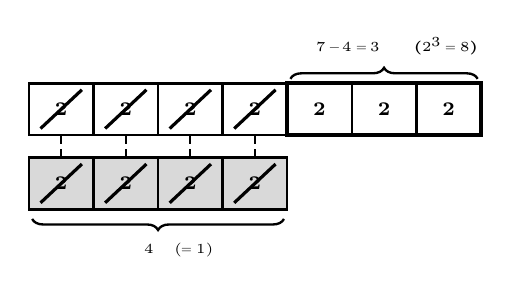
\begin{tikzpicture}[x=0.82cm, y=0.82cm, every node/.style={font=\scriptsize, text=black}]
      % Compact visual diagram showing 1-to-1 pairing & cancellation of first 4 pairs
      \foreach \i in {0,...,6}{
        \draw[black, line width=0.9pt, fill=white] (\i, 1.35) rectangle (\i+1, 2.15);
        \node at (\i+0.5, 1.75) {$\mathbf{2}$};
      }
      \foreach \i in {0,...,3}{
        \draw[black, line width=0.9pt, fill=headgray] (\i, 0.20) rectangle (\i+1, 1.00);
        \node at (\i+0.5, 0.60) {$\mathbf{2}$};
        % 1-to-1 cancel slash & vertical connector
        \draw[black, densely dashed, line width=0.75pt] (\i+0.5, 1.00) -- (\i+0.5, 1.35);
        \draw[black, line width=1.15pt] (\i+0.18, 1.45) -- (\i+0.82, 2.05);
        \draw[black, line width=1.15pt] (\i+0.18, 0.30) -- (\i+0.82, 0.90);
      }
      % Highlight the 3 remaining boxes
      \draw[black, line width=1.5pt] (4.0, 1.35) rectangle (7.0, 2.15);
      \draw[black, decorate, decoration={brace, amplitude=4pt, mirror}, line width=0.85pt] (0.05, 0.05) -- (3.95, 0.05)
        node[midway, below=5pt, font=\tiny] {សម្រួលអស់ $4$ គូ ($=1$)};
      \draw[black, decorate, decoration={brace, amplitude=4pt}, line width=0.85pt] (4.05, 2.22) -- (6.95, 2.22)
        node[midway, above=5pt, font=\tiny] {\textbf{នៅសល់ $7-4 = 3$ កត្តា ($2^3=8$)}};
    \end{tikzpicture}
  \end{minipage}%
  \hfill
  \begin{minipage}[c]{9.65cm}
    \raggedright\fontsize{8.0pt}{12.0pt}\selectfont
    \textbf{១) លំនាំទូទៅ ($a\neq 0$, $m>n$)៖} ព្រោះកត្តា $a$ នៅភាគបែង $n$ ដង ត្រូវបានសម្រួលនឹង $a$ នៅភាគយក $n$ ដង ($\frac{a}{a}=1$) នោះនៅសល់ $a$ គុណគ្នា $(m-n)$ កត្តា៖\par\vspace{4pt}
    {\centering\fbox{\strut\hspace{6pt}$\dfrac{a^m}{a^n} = a^{\underline{\hspace{0.6cm}} - \underline{\hspace{0.6cm}}}$ \quad ($a \neq 0$)\hspace{6pt}}\par}\vspace{5pt}
    \textbf{២) បញ្ជាក់កំហុសអន្ទាក់ \en{Ulusoy (2019)}៖} ហេតុអ្វី $\dfrac{2^7}{2^4}$ \textbf{មិនស្មើ} $1^3$ ហើយ \textbf{មិនស្មើ} $2^{\frac{7}{4}}$?\\
    $\underline{\hspace{9.4cm}}$\\[4pt]
    $\underline{\hspace{9.4cm}}$\\[4pt]
    \textbf{៣) ដោះស្រាយ \en{E1} ឃ្លាំងទិន្នន័យ \en{NGS}៖} $2^7\unit{MB} \div 2^4\unit{MB} = 2^{\underline{\hspace{0.4cm}}} = \underline{\hspace{0.6cm}}\text{ កញ្ចប់!}$
  \end{minipage}
\end{tcolorbox}

\vspace{8pt}
\begin{tcolorbox}[
  enhanced, sharp corners, colback=white, colframe=black,
  boxrule=0.95pt, boxsep=1pt, top=5pt, bottom=5pt, left=6.5pt, right=6.5pt
]
  \raggedright\fontsize{7.85pt}{11.4pt}\selectfont
  \textbf{ប្រអប់ផ្ទៀងផ្ទាត់ក្រុម (មុនបន្តទៅ \en{E2 Act 2})៖}\\[3pt]
  \chkbox\ បន្ទះកាត់ $2^7$ មាន \textbf{៧ កត្តាពេញ} ($7.00\unit{cm}$ តាមបន្ទាត់ \en{cm}, \textit{មិនមែន ៦ កត្តាដូចកំហុសបោះពុម្ពទំ.១៦ ទេ!})\\[2pt]
  \chkbox\ បន្ទះកាត់ $3^7$ ($7.00\unit{cm}$) ផ្ទឹមលើ $3^5$ ($5.00\unit{cm}$) សល់ $2.00\unit{cm} \Rightarrow 3^2 = 9$ \quad \chkbox\ ក្រុមយល់ច្បាស់ថា \textbf{គោលរក្សាដដែល និងដកនិទស្សន្ត}!
\end{tcolorbox}

\clearpage

% ============================================================================
% ទំព័រទី ២៖ សម្ភារៈ E2 សកម្មភាព 2 — Dual POE 2A/2B + ជណ្ដើរស្វ័យគុណ + ដែនកំណត់ a≠0
% ============================================================================
\pagebanner{សម្ភារៈទី ២៖ ពិសោធន៍ \enbf{POE 2A--2B} និងជណ្ដើរស្វ័យគុណ \enbf{(}និទស្សន្តសូន្យ និងអវិជ្ជមាន \enbf{a$\neq$0)}}{ទំព័រ ២/៦ \en{-- E2 Act 2}}

% --- ផ្នែកទី ១៖ Dual POE 2A (m = n) & POE 2B (m < n) ---
\noindent
\begin{tcolorbox}[
  enhanced, sharp corners, colback=white, colframe=black,
  width=9.28cm, equal height group=poe2row, nobeforeafter,
  boxrule=1.05pt, boxsep=1pt, top=3.5pt, bottom=4pt, left=5.5pt, right=5.5pt,
  title={\textbf{\en{POE 2A} ($m=n$)៖ តើ $a^0$ ស្មើ $0$ ឬ $1$? ($\dfrac{a^4}{a^4},\; a\neq 0$)}},
  colbacktitle=headgray, coltitle=black, fonttitle=\fontsize{8.2pt}{11.2pt}\selectfont
]
  \centering
  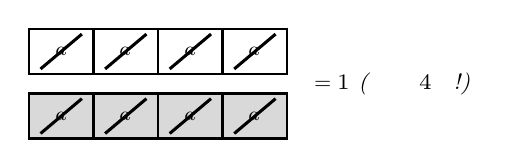
\begin{tikzpicture}[x=0.82cm, y=0.82cm, every node/.style={font=\scriptsize, text=black}]
    \foreach \i in {0,...,3}{
      \draw[black, line width=0.9pt, fill=white] (\i, 1.15) rectangle (\i+1, 1.85);
      \node at (\i+0.5, 1.50) {$a$};
      \draw[black, line width=0.9pt, fill=headgray] (\i, 0.15) rectangle (\i+1, 0.85);
      \node at (\i+0.5, 0.50) {$a$};
      \draw[black, line width=1.1pt] (\i+0.18, 1.23) -- (\i+0.82, 1.77);
      \draw[black, line width=1.1pt] (\i+0.18, 0.23) -- (\i+0.82, 0.77);
    }
    \node[right=4pt, font=\footnotesize] at (4.10, 1.00) {$= 1$ \textit{(អស់ទាំង $4$ គូ!)} };
  \end{tikzpicture}
  \par\vspace{3pt}\raggedright\fontsize{7.85pt}{11.4pt}\selectfont
  \textbf{\en{P} -- ទស្សន៍ទាយមុនគណនា៖} ចំពោះ $a\neq 0$ តើ $a^0$ ស្មើប៉ុន្មាន?\\
  \chkbox~$0$ \qquad \chkbox~$1$ \qquad \chkbox~$a$ \qquad \textit{(ហេតុផល៖ $\underline{\hspace{2.9cm}}$)}\\[4pt]
  \textbf{\en{O} -- សង្កេតតាម ២ វិធី៖}\\[2pt]
  $\bullet$ \textbf{វិធីសម្រួលកត្តា៖} $\dfrac{a^4}{a^4} = \dfrac{a\cdot a\cdot a\cdot a}{a\cdot a\cdot a\cdot a} = \underline{\hspace{0.75cm}}$ \textit{(ភាគយក=ភាគបែង)}\\[3pt]
  $\bullet$ \textbf{វិធីរូបមន្តដក៖} $\dfrac{a^4}{a^4} = a^{4-4} = a^{\rule{0.42cm}{0.5pt}}$\\[5pt]
  \textbf{\en{E} -- ពន្យល់សន្និដ្ឋាន៖} ព្រោះកន្សោមទាំងពីរស្មើគ្នា $\Rightarrow$\par\vspace{4pt}
  {\centering\fbox{\strut\hspace{5pt}\textbf{$a^0 = \underline{\hspace{0.55cm}}$ \quad ($a \neq 0$)}\hspace{5pt}}\par}\vspace{5pt}
  \begin{tcolorbox}[enhanced, sharp corners, colback=panelgray, colframe=black, boxrule=0.7pt, boxsep=1pt, top=3.5pt, bottom=3.5pt, left=4.5pt, right=4.5pt]
    \raggedright\fontsize{7.55pt}{10.8pt}\selectfont
    \textbf{ប្រយ័ត្នអន្ទាក់សញ្ញាដក (\en{Ulusoy, 2019})៖}\\
    $(-5)^0 = \underline{\hspace{0.5cm}}$ \textit{(វង់ក្រចក)} \quad តែ \quad $-5^0 = -(5^0) = \underline{\hspace{0.5cm}}$!\\[2pt]
    \textit{មូលហេតុ៖} $\underline{\hspace{7.0cm}}$
  \end{tcolorbox}
\end{tcolorbox}%
\hfill
\begin{tcolorbox}[
  enhanced, sharp corners, colback=white, colframe=black,
  width=9.28cm, equal height group=poe2row, nobeforeafter,
  boxrule=1.05pt, boxsep=1pt, top=4.5pt, bottom=4.5pt, left=5.5pt, right=5.5pt,
  title={\textbf{\en{POE 2B} ($m<n$)៖ តើ $a^{-n}$ ជាលេខដក ឬភាគច្រាស? ($\dfrac{a^2}{a^4},\; a\neq 0$)}},
  colbacktitle=headgray, coltitle=black, fonttitle=\fontsize{8.2pt}{11.2pt}\selectfont
]
  \centering
  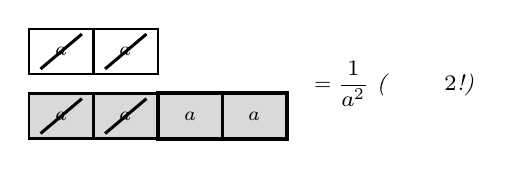
\begin{tikzpicture}[x=0.82cm, y=0.82cm, every node/.style={font=\scriptsize, text=black}]
    \foreach \i in {0,1}{
      \draw[black, line width=0.9pt, fill=white] (\i, 1.15) rectangle (\i+1, 1.85);
      \node at (\i+0.5, 1.50) {$a$};
      \draw[black, line width=1.1pt] (\i+0.18, 1.23) -- (\i+0.82, 1.77);
    }
    \foreach \i in {0,...,3}{
      \draw[black, line width=0.9pt, fill=headgray] (\i, 0.15) rectangle (\i+1, 0.85);
      \node at (\i+0.5, 0.50) {$a$};
    }
    \foreach \i in {0,1}{
      \draw[black, line width=1.1pt] (\i+0.18, 0.23) -- (\i+0.82, 0.77);
    }
    \draw[black, line width=1.45pt] (2.0, 0.15) rectangle (4.0, 0.85);
    \node[right=4pt, font=\footnotesize] at (4.10, 1.00) {$= \dfrac{1}{a^2}$ \textit{(សល់ក្រោម $2$!)}};
  \end{tikzpicture}
  \par\vspace{3pt}\raggedright\fontsize{7.85pt}{11.4pt}\selectfont
  \textbf{\en{P} -- ទស្សន៍ទាយមុនគណនា៖} ចំពោះ $2^{-2}$ តើស្មើប៉ុន្មាន?\\
  \chkbox~$-4$ \qquad \chkbox~$-\dfrac{1}{4}$ \qquad \chkbox~$\dfrac{1}{4}$ \qquad \textit{(ហេតុផល៖ $\underline{\hspace{2.5cm}}$)}\\[4pt]
  \textbf{\en{O} -- សង្កេតតាម ២ វិធី៖}\\[2pt]
  $\bullet$ \textbf{វិធីសម្រួលកត្តា៖} $\dfrac{a^2}{a^4} = \dfrac{\stk{a}\cdot\stk{a}}{\stk{a}\cdot\stk{a}\cdot a\cdot a} = \dfrac{1}{a^{\rule{0.40cm}{0.5pt}}}$ \textit{(នៅភាគបែង!)}\\[3pt]
  $\bullet$ \textbf{វិធីរូបមន្តដក៖} $\dfrac{a^2}{a^4} = a^{2-4} = a^{\rule{0.52cm}{0.5pt}}$\\[5pt]
  \textbf{\en{E} -- ពន្យល់សន្និដ្ឋាន៖} និទស្សន្តដកបង្ហាញ \textbf{ចំនួនច្រាស} មិនមែនលេខដកទេ៖\par\vspace{4pt}
  {\centering\fbox{\strut\hspace{4pt}\textbf{$a^{-n} = \dfrac{1}{a^{\rule{0.38cm}{0.5pt}}}$} \quad និងបញ្ច្រាស \quad \textbf{$\dfrac{1}{a^{-n}} = a^{\rule{0.38cm}{0.5pt}}$ ($a \neq 0$)}\hspace{4pt}}\par}\vspace{5pt}
  \begin{tcolorbox}[enhanced, sharp corners, colback=panelgray, colframe=black, boxrule=0.7pt, boxsep=1pt, top=3.5pt, bottom=3.5pt, left=4.5pt, right=4.5pt]
    \raggedright\fontsize{7.55pt}{10.8pt}\selectfont
    \textbf{សាកល្បងភ្លាម ($y\neq 0$)៖} $2^{-2} = \underline{\hspace{0.75cm}}$ \quad | \quad $\dfrac{1}{y^{-2}} = \underline{\hspace{0.75cm}}$!\\[2pt]
    \textit{ផ្ទៀង៖} តើ $(-2)^{-2} = \frac{1}{(-2)^2} = \underline{\hspace{0.6cm}}$ ជាលេខវិជ្ជមានឬអវិជ្ជមាន?
  \end{tcolorbox}
\end{tcolorbox}

\vspace{7pt}

% --- ផ្នែកទី ២៖ ជណ្ដើរស្វ័យគុណ (Exponent Ladder: a^3 -> a^{-2} ÷ a) ---
\begin{tcolorbox}[
  enhanced, sharp corners, colback=white, colframe=black,
  boxrule=1.05pt, boxsep=1pt, top=4pt, bottom=5pt, left=6pt, right=6pt,
  title={\textbf{ជណ្ដើរស្វ័យគុណ (\en{Exponent Ladder}: $a^3 \to a^{-2}$, ចែកនឹង $a$ តាមលំដាប់ \en{-- Ellis et al., 2013})}},
  colbacktitle=headgray, coltitle=black, fonttitle=\fontsize{8.2pt}{11.2pt}\selectfont
]
  \noindent
  \begin{minipage}[c]{10.50cm}
    \centering
    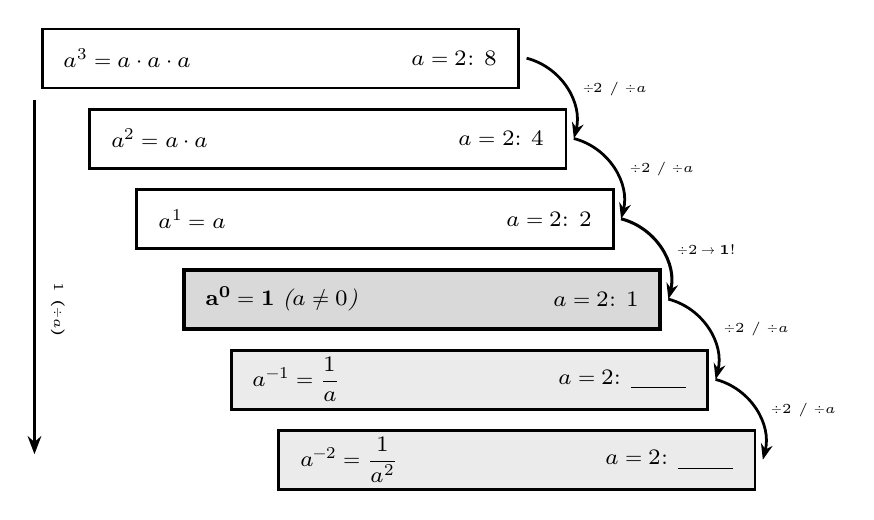
\begin{tikzpicture}[x=1cm, y=1cm, every node/.style={font=\footnotesize, text=black}]
      % Step boxes from a^3 down to a^{-2}
      \draw[black, line width=1.0pt, fill=white] (0.15, 5.20) rectangle (6.20, 5.95);
      \node[anchor=west] at (0.30, 5.58) {$a^3 = a\cdot a\cdot a$};
      \node[anchor=east] at (6.05, 5.58) {គោល $a=2$: \textbf{$8$}};

      \draw[black, line width=1.0pt, fill=white] (0.75, 4.18) rectangle (6.80, 4.93);
      \node[anchor=west] at (0.90, 4.56) {$a^2 = a\cdot a$};
      \node[anchor=east] at (6.65, 4.56) {គោល $a=2$: \textbf{$4$}};

      \draw[black, line width=1.0pt, fill=white] (1.35, 3.16) rectangle (7.40, 3.91);
      \node[anchor=west] at (1.50, 3.54) {$a^1 = a$};
      \node[anchor=east] at (7.25, 3.54) {គោល $a=2$: \textbf{$2$}};

      % Highlighted a^0 = 1 step
      \draw[black, line width=1.45pt, fill=headgray] (1.95, 2.14) rectangle (8.00, 2.89);
      \node[anchor=west] at (2.10, 2.52) {$\mathbf{a^0 = 1}$ \textit{($a\neq 0$)}};
      \node[anchor=east] at (7.85, 2.52) {គោល $a=2$: \textbf{$1$}};

      \draw[black, line width=1.0pt, fill=panelgray] (2.55, 1.12) rectangle (8.60, 1.87);
      \node[anchor=west] at (2.70, 1.50) {$a^{-1} = \dfrac{1}{a}$};
      \node[anchor=east] at (8.45, 1.50) {គោល $a=2$: \underline{\hspace{0.7cm}}};

      \draw[black, line width=1.0pt, fill=panelgray] (3.15, 0.10) rectangle (9.20, 0.85);
      \node[anchor=west] at (3.30, 0.48) {$a^{-2} = \dfrac{1}{a^2}$};
      \node[anchor=east] at (9.05, 0.48) {គោល $a=2$: \underline{\hspace{0.7cm}}};

      % Curved arrows showing ÷ a / exponent - 1 at each step
      \draw[black, line width=1.0pt, -{Stealth[length=2mm]}] (6.30, 5.58) to[bend left=45] node[right=2pt, font=\tiny] {$\div 2$ / $\div a$} (6.90, 4.56);
      \draw[black, line width=1.0pt, -{Stealth[length=2mm]}] (6.90, 4.56) to[bend left=45] node[right=2pt, font=\tiny] {$\div 2$ / $\div a$} (7.50, 3.54);
      \draw[black, line width=1.1pt, -{Stealth[length=2mm]}] (7.50, 3.54) to[bend left=45] node[right=2pt, font=\tiny] {$\div 2 \to \mathbf{1}$!} (8.10, 2.52);
      \draw[black, line width=1.0pt, -{Stealth[length=2mm]}] (8.10, 2.52) to[bend left=45] node[right=2pt, font=\tiny] {$\div 2$ / $\div a$} (8.70, 1.50);
      \draw[black, line width=1.0pt, -{Stealth[length=2mm]}] (8.70, 1.50) to[bend left=45] node[right=2pt, font=\tiny] {$\div 2$ / $\div a$} (9.30, 0.48);

      % Left downward arrow showing Exponent - 1
      \draw[black, line width=1.15pt, -{Stealth[length=2.3mm]}] (0.05, 5.05) -- (0.05, 0.55)
        node[midway, sloped, above=2pt, font=\tiny] {\textbf{និទស្សន្តថយម្ដង $1$ ($\div a$)}};
    \end{tikzpicture}
  \end{minipage}%
  \hfill
  \begin{minipage}[c]{7.95cm}
    \raggedright\fontsize{7.7pt}{11.0pt}\selectfont
    \textbf{តារាងអនុវត្តលំនាំ $\div a$ សម្រាប់ $a=3$ និង $a=10$៖}\\[3pt]
    \renewcommand{\arraystretch}{1.28}
    \begin{tabular}{|C{1.55cm}|C{2.45cm}|C{2.75cm}|}
      \hline
      \cellcolor{headgray}\textbf{និទស្សន្ត} & \cellcolor{headgray}\textbf{គោល $a=3$} & \cellcolor{headgray}\textbf{គោល $a=10$} \\ \hline
      $a^3$ & $27$ & $1000$ \\ \hline
      $a^2$ & $9$ & $100$ \\ \hline
      $a^1$ & $3$ & $10$ \\ \hline
      $a^0$ & $\underline{\hspace{0.9cm}}$ \textit{($3\div 3$)} & $\underline{\hspace{0.9cm}}$ \textit{($10\div 10$)} \\ \hline
      $a^{-1}$ & $\underline{\hspace{0.9cm}}$ \textit{($1\div 3$)} & $\underline{\hspace{0.9cm}}$ \textit{($1\div 10$)} \\ \hline
      $a^{-2}$ & $\underline{\hspace{0.9cm}}$ & $\underline{\hspace{0.9cm}}$ \\ \hline
    \end{tabular}\\[5pt]
    \textbf{សំណួរគិត ($a>0$)៖} នៅពេលនិទស្សន្តចុះក្រោមសូន្យ ($-1, -2$) តើតម្លៃក្លាយជាលេខដកឬទេ? \chkbox~ទេ (ក្លាយជាប្រភាគវិជ្ជមានកាន់តែតូច!)
  \end{minipage}
\end{tcolorbox}

\vspace{7pt}

% --- ផ្នែកទី ៣៖ ប្រអប់ការពារដែនកំណត់ a ≠ 0 (បំពេញចន្លោះសៀវភៅទំ.១៦) & សាកល្បងរហ័ស ---
\noindent
\begin{minipage}[t]{11.45cm}
  \begin{tcolorbox}[
    enhanced, sharp corners, colback=panelgray, colframe=black,
    boxrule=1.2pt, borderline={0.5pt}{2pt}{black},
    equal height group=domainrow,
    boxsep=1pt, top=4.5pt, bottom=4.5pt, left=6pt, right=6pt,
    title={\textbf{ប្រអប់ការពារដែនកំណត់ $a\neq 0$ (កែបំពេញសៀវភៅទំ.១៦)}},
    colbacktitle=headgray, coltitle=black, fonttitle=\fontsize{8.1pt}{11.0pt}\selectfont
  ]
    \raggedright\fontsize{7.75pt}{11.3pt}\selectfont
    \textbf{ហេតុអ្វីត្រូវសរសេរ $a \neq 0$ គ្រប់រូបមន្ត?} \textit{(សៀវភៅទំ.១៦ ខកខានសរសេរ $a\neq 0$ លើ $a^{-n}=\frac{1}{a^n}$)}\\[3pt]
    $\bullet$ $\dfrac{a^m}{a^n} = a^{m-n}$ ($a\neq 0$)៖ បើ $a=0$ នោះ $\dfrac{0^m}{0^n} = \dfrac{0}{0}$ \textbf{គ្មានន័យ} (ហាមចែកនឹង $0$!)។\\[2pt]
    $\bullet$ $a^0 = 1$ ($a\neq 0$)៖ $0^0$ មិនកំណត់! \quad $\bullet$ $a^{-n} = \dfrac{1}{a^n}$ និង $\dfrac{1}{a^{-n}} = a^n$ ($a\neq 0$)៖ $0^{-2} = \dfrac{1}{0^2}$ \textbf{គ្មានន័យ}!\\[3pt]
    \textbf{ត្រួតពិនិត្យ៖} តើ $0^{-4}$ ស្មើ $0$ ឬគ្មានន័យ? \chkbox~ស្មើ $0$ \quad \chkbox~\textbf{គ្មានន័យ} (ព្រោះចែកនឹង $0$)
  \end{tcolorbox}
\end{minipage}%
\hfill
\begin{minipage}[t]{7.15cm}
  \begin{tcolorbox}[
    enhanced, sharp corners, colback=white, colframe=black,
    equal height group=domainrow,
    boxrule=1.05pt, boxsep=1pt, top=4.5pt, bottom=4.5pt, left=5.5pt, right=5.5pt,
    title={\textbf{ផ្ទៀងរហ័ស ៣០ វិនាទី (\en{E2 Check})}},
    colbacktitle=headgray, coltitle=black, fonttitle=\fontsize{8.1pt}{11.0pt}\selectfont
  ]
    \raggedright\fontsize{7.85pt}{12.0pt}\selectfont
    ១) $2^0 = \underline{\hspace{0.85cm}}$ \qquad ២) $2^{-2} = \underline{\hspace{0.85cm}}$\\[2pt]
    ៣) $\dfrac{1}{5^{-2}} = \underline{\hspace{0.85cm}}$ \quad ៤) $(-7)^0 = \underline{\hspace{0.85cm}}$\\[2pt]
    ៥) $-7^0 = \underline{\hspace{0.85cm}}$ \quad ៦) $\dfrac{y^8}{y^{-2}} = \underline{\hspace{0.85cm}}$ ($y\neq 0$)
  \end{tcolorbox}
\end{minipage}

\vspace{9pt}
\begin{tcolorbox}[
  enhanced, sharp corners, colback=panelgray, colframe=black,
  boxrule=1.0pt, boxsep=1pt, top=5pt, bottom=5pt, left=6pt, right=6pt
]
  \raggedright\fontsize{7.9pt}{11.5pt}\selectfont
  \textbf{សង្ខេបរូបមន្តស្នូលទាំង ៤ (សៀវភៅទំព័រ ១៦ + កែបំពេញដែនកំណត់ $a\neq 0$)៖}\\[3pt]
  \textbf{១.} $\dfrac{a^m}{a^n} = a^{m-n}$ ($a\neq 0$) \qquad
  \textbf{២.} $a^0 = 1$ ($a\neq 0$) \qquad
  \textbf{៣.} $a^{-n} = \dfrac{1}{a^n}$ ($a\neq 0$) \qquad
  \textbf{៤.} $\dfrac{1}{a^{-n}} = a^n$ ($a\neq 0$)\\[3pt]
  \textbf{សេចក្ដីសន្និដ្ឋានសិស្ស៖} ហេតុអ្វី $a^0 = 1$ មិនមែន $0$ ហើយ $a^{-2} = \frac{1}{a^2}$ មិនមែន $-a^2$? $\underline{\hspace{7.8cm}}$
\end{tcolorbox}

\clearpage

% ============================================================================
% ទំព័រទី ៣៖ E3/E4 — ធនាគារហេតុផល ①–⑤ + កាតប្រៀបធៀប (-2)^6 vs -2^6 + កាត [tracing] ៣ ជំហាន
% ============================================================================
\pagebanner{សម្ភារៈទី ៣៖ ធនាគារហេតុផល \enbf{(}\cnum{1}\enbf{--}\cnum{5}\enbf{)} និងកាតស៊ើបអង្កេត \enbf{E4 [tracing]} ៣ ជំហាន}{ទំព័រ ៣/៦ \en{-- E3 \& E4}}

% --- ផ្នែកទី ១៖ ធនាគារហេតុផលផ្លូវការ ①–⑤ (E3 Explain) ---
\begin{tcolorbox}[
  enhanced, sharp corners, colback=white, colframe=black,
  boxrule=1.1pt, boxsep=1pt, top=4pt, bottom=4.5pt, left=5.5pt, right=5.5pt,
  title={\textbf{ធនាគារហេតុផលផ្លូវការ \cnum{1}--\cnum{5} (\en{Warrant Bank -- Vest et al., 2022}) និងវិធានទូទៅ (ទំ.១៦, $a\neq 0$)}},
  colbacktitle=headgray, coltitle=black, fonttitle=\fontsize{8.2pt}{11.2pt}\selectfont
]
  \renewcommand{\arraystretch}{1.18}
  \begin{tabular}{|C{0.9cm}|L{4.25cm}|L{7.00cm}|L{4.95cm}|}
    \hline
    \cellcolor{panelgray}\textbf{លេខ} & \cellcolor{panelgray}\textbf{ឈ្មោះវិធាន / លក្ខណៈ} & \cellcolor{panelgray}\textbf{រូបមន្តគណិតវិទ្យា និងដែនកំណត់} & \cellcolor{panelgray}\textbf{ប្រយ័ត្នអន្ទាក់ទូទៅ} \\ \hline
    \cnum{1} & \textbf{ចែកគោលដូចគ្នា} & $\dfrac{a^m}{a^n} = a^{m-n}$ \quad ($a\neq 0,\; m,n \in \mathbb{Z}$) & កុំចែកគោល ($\frac{a}{a}$) ឬចែកនិទស្សន្ត! \\ \hline
    \cnum{2} & \textbf{និទស្សន្តសូន្យ} & $a^0 = 1$ \quad ($a \neq 0$) & មិនស្មើ $0$ ទេ; $-a^0 = -1$! \\ \hline
    \cnum{3} & \textbf{និទស្សន្តអវិជ្ជមាន / បញ្ច្រាស} & $a^{-n} = \dfrac{1}{a^n}$ \;\;និង\;\; $\dfrac{1}{a^{-n}} = a^n$ \quad ($a\neq 0$) & មិនមែនលេខដក ($-a^n$) ទេ! \\ \hline
    \cnum{4} & \textbf{ដករ៉ឺឡាទីប \& និទស្សន្តលាក់} & $m - (-n) = m + n$ \;\;និង\;\; $x = x^1$ & ប្រយ័ត្ន $-(-2)=+2$ និង $x=x^1$! \\ \hline
    \cnum{5} & \textbf{ផ្ដុំមេគុណ / គុណ ២.២} & ផ្ដុំមេគុណ-គោលដូចគ្នា; $a^m\cdot a^n = a^{m+n}$ & បំបែកលេខ-អថេរឱ្យដាច់តាមក្រុម! \\ \hline
  \end{tabular}
\end{tcolorbox}

\vspace{6pt}

% --- ផ្នែកទី ២៖ លំហាត់គំរូ ក, ខ (ទំ.១៦) & កាតប្រៀបធៀប (-2)^6 vs -2^6 ---
\noindent
\begin{minipage}[t]{8.50cm}
  \begin{tcolorbox}[
    enhanced, sharp corners, colback=white, colframe=black,
    equal height group=e4toprow,
    boxrule=1.0pt, boxsep=1pt, top=4pt, bottom=4pt, left=5.5pt, right=5.5pt,
    title={\textbf{លំហាត់គំរូ ក, ខ (សៀវភៅទំ.១៦) \en{--} បំពេញសំអាង}},
    colbacktitle=headgray, coltitle=black, fonttitle=\fontsize{8.0pt}{10.8pt}\selectfont
  ]
    \raggedright\fontsize{7.8pt}{11.8pt}\selectfont
    \textbf{ក.} $\dfrac{10^8}{10^6} = 10^{\underline{\hspace{0.4cm}}-\underline{\hspace{0.4cm}}} = 10^{\underline{\hspace{0.35cm}}} = \underline{\hspace{0.9cm}}$ \hfill [\blankcnum]\\[5pt]
    \textbf{ខ.} $\dfrac{(-2)^6}{(-2)^5} = (-2)^{\underline{\hspace{0.4cm}}-\underline{\hspace{0.4cm}}} = (-2)^{\underline{\hspace{0.35cm}}} = \underline{\hspace{0.75cm}}$ \hfill [\blankcnum, \blankcnum]\\[4pt]
    \textit{សម្គាល់៖ ក្នុង \textbf{ខ.} គោលគឺ $(-2)$ ជាប់វង់ក្រចកទាំងអស់!}
  \end{tcolorbox}
\end{minipage}%
\hfill
\begin{minipage}[t]{10.10cm}
  \begin{tcolorbox}[
    enhanced, sharp corners, colback=panelgray, colframe=black,
    equal height group=e4toprow,
    boxrule=1.0pt, boxsep=1pt, top=4pt, bottom=4pt, left=5.5pt, right=5.5pt,
    title={\textbf{កាតប្រៀបធៀបអន្ទាក់វង់ក្រចក៖ $(-2)^6$ \en{vs} $-2^6$ (\en{Olson et al., 2011})}},
    colbacktitle=headgray, coltitle=black, fonttitle=\fontsize{8.0pt}{10.8pt}\selectfont
  ]
    \renewcommand{\arraystretch}{1.15}
    \fontsize{7.55pt}{10.8pt}\selectfont
    \begin{tabular}{|L{4.45cm}|L{4.45cm}|}
      \hline
      \cellcolor{white}\textbf{១) មានវង់ក្រចក៖ $(-2)^6$} & \cellcolor{white}\textbf{២) គ្មានវង់ក្រចក៖ $-2^6$} \\ \hline
      គោលគឺ $\mathbf{(-2)}$ ទាំងសញ្ញាដក៖\newline $(-2)(-2)(-2)(-2)(-2)(-2)$\newline $= \mathbf{+64}$ \quad \textit{(គូ $\to$ វិជ្ជមាន)} &
      គោលគឺ $\mathbf{2}$ សញ្ញាដកនៅក្រៅ៖\newline $-(2\cdot 2\cdot 2\cdot 2\cdot 2\cdot 2)$\newline $= \mathbf{-64}$ \quad \textit{(ដាក់ដកខាងមុខ!)} \\ \hline
    \end{tabular}
    \par\vspace{3pt}
    \textbf{ផ្ទៀងសញ្ញាសូន្យ៖} $(-2)^0 = \underline{\hspace{0.55cm}}$ \quad \textbf{vs} \quad $-2^0 = \underline{\hspace{0.55cm}}$ \textit{(ខុសគ្នា!)}
  \end{tcolorbox}
\end{minipage}

\vspace{7pt}

% --- ផ្នែកទី ៣៖ កាតស៊ើបអង្កេត B&W [tracing] ៣ ជំហាន — លំហាត់គំរូ គ (ទំ.១៦) ---
\begin{tcolorbox}[
  enhanced, sharp corners, colback=white, colframe=black,
  boxrule=1.2pt, boxsep=1pt, top=4.5pt, bottom=5pt, left=6pt, right=6pt,
  title={\textbf{កាតស៊ើបអង្កេត \en{E4} ៣ ជំហាន (\en{Monochrome B\&W [tracing]} -- \en{Yeo \& Tzeng, 2019})៖ លំហាត់គំរូ គ (ទំ.១៦)}},
  colbacktitle=headgray, coltitle=black, fonttitle=\fontsize{8.2pt}{11.2pt}\selectfont
]
  \centering\fontsize{8.1pt}{11.5pt}\selectfont
  \textbf{ប្រធាន៖} គណនាកន្សោម $\dfrac{\frac{5}{4}x^3 y^8}{-5x y^{-2}}$ \textit{($x\neq 0,\; y\neq 0$)} ដោយប្រើសញ្ញាកូដ ស-ខ្មៅ ៣ ក្រុម និងគូសដានម្រាមដៃ \en{[tracing]}។\\[4pt]

  % --- ដ្យាក្រាម B&W [tracing] កាត់បន្ថយបន្ទុកគិត ---
  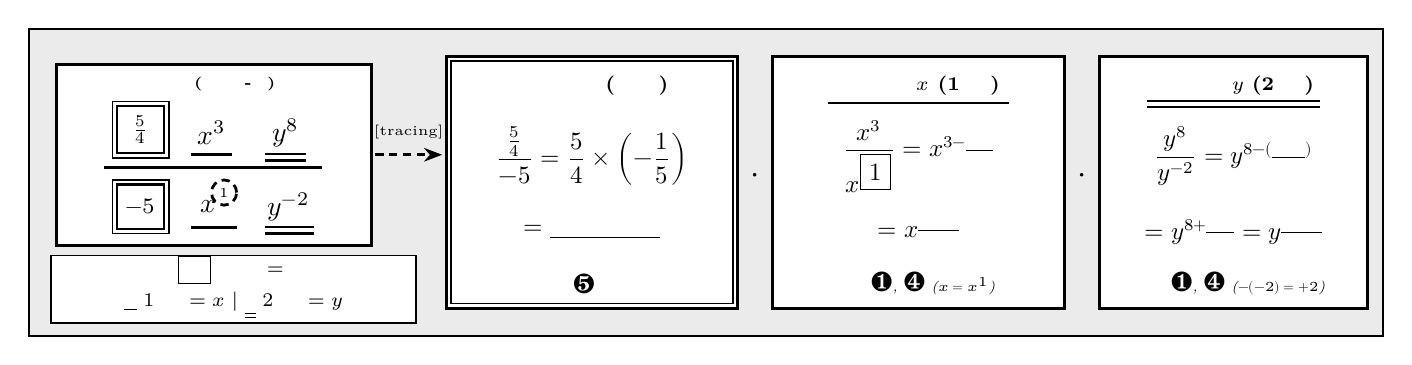
\begin{tikzpicture}[x=1cm, y=1cm, every node/.style={text=black}]
    % Background schematic box
    \draw[black, line width=0.8pt, fill=panelgray] (0, 0.20) rectangle (17.2, 4.10);

    % Left original expression in zoom box
    \draw[black, line width=1.1pt, fill=white] (0.35, 1.35) rectangle (4.35, 3.65);
    \node[font=\tiny] at (2.35, 3.40) {\textbf{កន្សោមដើម (គូសក្រុម ស-ខ្មៅ)}};

    % Coefficient double-box
    \draw[black, line width=0.9pt] (1.12, 2.52) rectangle (1.72, 3.12);
    \draw[black, line width=0.5pt] (1.06, 2.46) rectangle (1.78, 3.18);
    \node[font=\footnotesize] at (1.42, 2.82) {$\frac{5}{4}$};
    \draw[black, line width=0.9pt] (1.12, 1.56) rectangle (1.72, 2.12);
    \draw[black, line width=0.5pt] (1.06, 1.50) rectangle (1.78, 2.18);
    \node[font=\footnotesize] at (1.42, 1.84) {$-5$};

    % x single-underline & circled hidden exponent 1
    \node[font=\normalsize] at (2.32, 2.78) {$x^3$};
    \draw[black, line width=1.2pt] (2.06, 2.50) -- (2.58, 2.50);
    \node[font=\normalsize] at (2.28, 1.84) {$x$};
    \draw[black, line width=1.0pt, densely dashed] (2.48, 2.02) circle (0.16);
    \node[font=\tiny] at (2.48, 2.02) {$1$};
    \draw[black, line width=1.2pt] (2.06, 1.58) -- (2.64, 1.58);

    % y double-underline & caution arrow on -2
    \node[font=\normalsize] at (3.26, 2.78) {$y^8$};
    \draw[black, line width=0.9pt] (3.00, 2.51) -- (3.52, 2.51);
    \draw[black, line width=0.9pt] (3.00, 2.43) -- (3.52, 2.43);
    \node[font=\normalsize] at (3.30, 1.84) {$y^{-2}$};
    \draw[black, line width=0.9pt] (3.00, 1.58) -- (3.62, 1.58);
    \draw[black, line width=0.9pt] (3.00, 1.50) -- (3.62, 1.50);

    % Fraction bar inside expression
    \draw[black, line width=1.0pt] (0.95, 2.34) -- (3.72, 2.34);

    % Legend strip under zoom box
    \draw[black, line width=0.6pt, fill=white] (0.28, 0.36) rectangle (4.92, 1.22);
    \node[font=\scriptsize, align=center, text width=4.4cm] at (2.60, 0.82) {\textbf{កូដ៖} \fbox{\rule{0pt}{3.5pt}\hspace{0.18cm}} ស៊ុមទ្វេ = មេគុណ\\[2pt] $\underline{\phantom{x}}$ \en{1} ជាន់ = $x$ \en{|} $\underline{\underline{\phantom{y}}}$ \en{2} ជាន់ = $y$};

    % Tracing arrows from zoom box to 3 target columns
    \draw[black, densely dashed, line width=1.05pt, -{Stealth[length=2.3mm]}] (4.40, 2.50) -- (5.25, 2.50)
      node[midway, above=2pt, font=\tiny] {\en{[tracing]}};

    % Column 1: Coefficients
    \draw[black, line width=1.1pt, fill=white] (5.30, 0.55) rectangle (9.00, 3.75);
    \draw[black, line width=0.6pt] (5.36, 0.61) rectangle (8.94, 3.69);
    \node[font=\scriptsize] at (7.15, 3.38) {\textbf{ក្រុម ១៖ មេគុណ (ស៊ុមទ្វេ)}};
    \node[font=\small] at (7.15, 2.48) {$\dfrac{\frac{5}{4}}{-5} = \dfrac{5}{4}\times \left(-\dfrac{1}{5}\right)$};
    \node[font=\small] at (7.15, 1.52) {$= \underline{\hspace{1.4cm}}$};
    \node[font=\tiny] at (7.15, 0.86) {\textit{សំអាង៖ \cnum{5} ផ្ដុំមេគុណ}};

    % Multiply dot between Col 1 & Col 2
    \node[font=\large] at (9.22, 2.20) {$\cdot$};

    % Column 2: Base x
    \draw[black, line width=1.1pt, fill=white] (9.45, 0.55) rectangle (13.15, 3.75);
    \node[font=\scriptsize] at (11.30, 3.38) {\textbf{ក្រុម ២៖ គោល $x$ (\en{1} ជាន់)}};
    \draw[black, line width=0.9pt] (10.15, 3.16) -- (12.45, 3.16);
    \node[font=\small] at (11.30, 2.48) {$\dfrac{x^3}{x^{\boxed{1}}} = x^{3-\underline{\hspace{0.35cm}}}$};
    \node[font=\small] at (11.30, 1.52) {$= x^{\underline{\hspace{0.5cm}}}$};
    \node[font=\tiny] at (11.30, 0.86) {\textit{សំអាង៖ \cnum{1}, \cnum{4} ($x=x^1$)}};

    % Multiply dot between Col 2 & Col 3
    \node[font=\large] at (13.38, 2.20) {$\cdot$};

    % Column 3: Base y
    \draw[black, line width=1.1pt, fill=white] (13.60, 0.55) rectangle (17.00, 3.75);
    \node[font=\scriptsize] at (15.30, 3.38) {\textbf{ក្រុម ៣៖ គោល $y$ (\en{2} ជាន់)}};
    \draw[black, line width=0.8pt] (14.20, 3.18) -- (16.40, 3.18);
    \draw[black, line width=0.8pt] (14.20, 3.11) -- (16.40, 3.11);
    \node[font=\small] at (15.30, 2.48) {$\dfrac{y^8}{y^{-2}} = y^{8-(\underline{\hspace{0.42cm}})}$};
    \node[font=\small] at (15.30, 1.52) {$= y^{8+\underline{\hspace{0.35cm}}} = y^{\underline{\hspace{0.5cm}}}$};
    \node[font=\tiny] at (15.30, 0.86) {\textit{សំអាង៖ \cnum{1}, \cnum{4} ($-(-2)=+2$)}};
  \end{tikzpicture}

  \par\vspace{6pt}\raggedright\fontsize{7.9pt}{11.6pt}\selectfont
  \textbf{ជំហាន ១ \en{--} គូសដាន \en{[tracing]} បំបែកក្រុម (\cnum{4}, \cnum{5})៖}
  $\dfrac{\frac{5}{4}x^3 y^8}{-5xy^{-2}} = \left(\dfrac{\frac{5}{4}}{-5}\right)\left(\dfrac{x^3}{x^{\underline{\hspace{0.35cm}}}}\right)\left(\dfrac{y^8}{y^{\underline{\hspace{0.45cm}}}}\right)$ \quad \textit{(ចុះដានម្រាមដៃពីឆ្វេងទៅស្ដាំ!)}\\[4pt]
  \textbf{ជំហាន ២ \en{--} គណនារួមបញ្ចូលគ្នា (\cnum{1}, \cnum{4})៖}
  $= \left(-\dfrac{1}{4}\right)\cdot x^{3-\underline{\hspace{0.35cm}}}\cdot y^{8-(\underline{\hspace{0.45cm}})} = -\dfrac{1}{4} x^{\underline{\hspace{0.35cm}}} y^{\underline{\hspace{0.45cm}}}$ \quad \textit{($x\neq 0,\; y\neq 0$)}\\[5pt]
  \begin{tcolorbox}[enhanced, sharp corners, colback=panelgray, colframe=black, boxrule=0.8pt, boxsep=1pt, top=3.5pt, bottom=3.5pt, left=5pt, right=5pt]
    \raggedright\fontsize{7.65pt}{11.0pt}\selectfont
    \textbf{ជំហាន ៣ \en{--} ផ្ទៀងក្រោយ \en{EIA Looking-Back} (ផ្ទៀង $\dfrac{y^8}{y^{-2}}$ តាម ២ របៀប)៖}\\[2pt]
    $\bullet$ \textbf{របៀបទី ១ (ដកនិទស្សន្ត \cnum{1}, \cnum{4})៖} $\dfrac{y^8}{y^{-2}} = y^{8-(-2)} = y^{8+2} = y^{\underline{\hspace{0.5cm}}}$\\[2pt]
    $\bullet$ \textbf{របៀបទី ២ (ច្រាសភាគបែង \cnum{3}, \cnum{5})៖} $\dfrac{y^8}{y^{-2}} = y^8 \cdot \dfrac{1}{y^{-2}} = y^8 \cdot y^{\underline{\hspace{0.4cm}}} = y^{8+2} = y^{\underline{\hspace{0.5cm}}}$ \quad \chkbox~លទ្ធផលដូចគ្នា ១០០\%!
  \end{tcolorbox}
\end{tcolorbox}

\vspace{6pt}
% --- ប្រអប់ហ្វឹកហាត់រួមគ្នា ៣០ វិនាទី (E4 Mini-Practice) ---
\begin{tcolorbox}[
  enhanced, sharp corners, colback=white, colframe=black, colbacktitle=headgray, coltitle=black,
  boxrule=0.9pt, titlerule=0.75pt, boxsep=1pt, top=5pt, bottom=5pt, left=7pt, right=7pt,
  toptitle=3.5pt, bottomtitle=3.5pt,
  title={\fontsize{8.8pt}{12pt}\selectfont\muol ហ្វឹកហាត់រួមគ្នា ៣០ វិនាទី \enbf{([tracing]} និង \cnum{1}\enbf{--}\cnum{5}\enbf{)}}
]
  \raggedright\fontsize{7.95pt}{11.8pt}\selectfont
  \textbf{១) ប្រៀបធៀបសញ្ញា និងវង់ក្រចក៖}\;
  $(-3)^4 = (-3)(-3)(-3)(-3) = \underline{\hspace{0.95cm}}$ \quad \textbf{ទល់នឹង} \quad $-3^4 = -(3\cdot 3\cdot 3\cdot 3) = \underline{\hspace{0.95cm}}$ \\[5pt]
  \textbf{២) បំបែកក្រុម ស-ខ្មៅ ($x\neq 0,\; y\neq 0$)៖}\;
  $\dfrac{6x^5 y^{-1}}{-2xy^3} = \left(\dfrac{6}{-2}\right)\left(\dfrac{x^5}{x^{\underline{\hspace{0.35cm}}}}\right)\left(\dfrac{y^{-1}}{y^3}\right) = \underline{\hspace{0.75cm}}\, x^{\underline{\hspace{0.45cm}}}\, y^{\underline{\hspace{0.55cm}}} = -\dfrac{3x^{\underline{\hspace{0.40cm}}}}{y^{\underline{\hspace{0.40cm}}}}$ \hfill \textbf{សំអាង៖} \blankcnum
\end{tcolorbox}

\clearpage

% ============================================================================
% ទំព័រទី ៤៖ សន្លឹកការងារក្រុម ៣ តួនាទី E5 Triad Relay (ប្រតិបត្តិ ក, ខ, គ, ឃ + បិទ E1)
% ============================================================================
\pagebanner{សម្ភារៈទី ៤៖ សន្លឹកការងារក្រុម ៣ តួនាទី \enbf{E5 Triad Relay --} ប្រតិបត្តិ ក\enbf{,} ខ\enbf{,} គ\enbf{,} ឃ \enbf{(x$\neq$0, y$\neq$0)}}{ទំព័រ ៤/៦ \en{-- E5 Evaluate}}

\begin{tcolorbox}[
  enhanced, sharp corners, colback=panelgray, colframe=black,
  boxrule=0.9pt, boxsep=1pt, top=3.5pt, bottom=3.5pt, left=5.5pt, right=5.5pt, after skip=5pt
]
  \fontsize{7.85pt}{11.0pt}\selectfont
  \textbf{ក្រុម៖} $\underline{\hspace{1.4cm}}$ \quad \textbf{តួនាទី ១ (\en{[tracing] \& Pause-Ask}):} $\underline{\hspace{2.8cm}}$ \quad \textbf{តួនាទី ២ (\cnum{1}--\cnum{5}):} $\underline{\hspace{2.8cm}}$ \quad \textbf{តួនាទី ៣ (\en{Pause-Review}):} $\underline{\hspace{2.8cm}}$\\[2pt]
  \textbf{ប្រតិបត្តិ (សៀវភៅទំព័រ ១៦)៖} សម្រួលកន្សោមខាងក្រោម \textit{($x\neq 0,\; y\neq 0$)} ដោយអនុវត្តវិធីវិលជុំ ៣ តួនាទី និងផ្ទៀងសំអាង \cnum{1}--\cnum{5} ជាមួយដៃគូ!
\end{tcolorbox}

% --- តារាងប្រតិបត្តិ ក, ខ, គ, ឃ តាម ៣ តួនាទី ---
{\setlength{\tabcolsep}{3pt}\renewcommand{\arraystretch}{1.34}
\fontsize{8.05pt}{11.8pt}\selectfont
\begin{tabular}{|C{2.05cm}|L{4.55cm}|L{6.75cm}|L{4.70cm}|}
  \hline
  \cellcolor{headgray}\centering\textbf{លំហាត់} &
  \cellcolor{headgray}\centering\textbf{តួនាទី ១៖ អ្នកគូសដាន \en{[tracing]}\newline \en{\& Pause-Ask!}} &
  \cellcolor{headgray}\centering\textbf{តួនាទី ២៖ អ្នកផ្គូផ្គងហេតុផល \cnum{1}--\cnum{5}\newline និងសម្រាយគណនា} &
  \cellcolor{headgray}\centering\arraybackslash\textbf{តួនាទី ៣៖ អ្នកត្រួតពិនិត្យ\newline \en{Pause-Review!}} \\ \hline

  % --- ប្រតិបត្តិ ក ---
  \textbf{ក.}\par\vspace{6pt} $\dfrac{x^9}{x^4}$ &
  \chkbox\ គូសបន្ទាត់ $1$ ជាន់ក្រោមគោល $x$ ទាំងលើ-ក្រោម។\par\vspace{3pt}
  \chkbox\ បញ្ជាក់ដែនកំណត់៖ $x \neq \underline{\hspace{0.4cm}}$។\par\vspace{3pt}
  \textit{សួរដៃគូ៖} ហេតុអ្វីមិនចែក $9\div 4$? &
  $\dfrac{x^9}{x^4} = x^{\underline{\hspace{0.45cm}} - \underline{\hspace{0.45cm}}} = \underline{\hspace{1.2cm}}$\par\vspace{20pt}
  \textbf{សំអាង៖} \blankcnum &
  \chkbox\ គោល $x$ រក្សាទុកដដែល\par\vspace{3pt}
  \chkbox\ ដកនិទស្សន្ត $9-4=5$ ត្រឹមត្រូវ\par\vspace{3pt}
  \chkbox\ មានលក្ខខណ្ឌ $x\neq 0$ \\[8pt] \hline

  % --- ប្រតិបត្តិ ខ (Pause-Ask! gate) ---
  \textbf{ខ.}\par\vspace{6pt} $\dfrac{\left(\frac{3}{2}\right)^2}{\left(\frac{3}{2}\right)^4}$ &
  \chkbox\ ព័ទ្ធរង្វង់គោលប្រភាគ $\left(\frac{3}{2}\right)$។\par\vspace{3pt}
  \chkbox\ \textbf{\en{Pause-Ask!}} តើនិទស្សន្ត $2-4$ ស្មើលេខអ្វី? ចុះ $\left(\frac{3}{2}\right)^{-2}$ ស្មើ $-\frac{9}{4}$ ឬ $\frac{4}{9}$? &
  $\dfrac{\left(\frac{3}{2}\right)^2}{\left(\frac{3}{2}\right)^4} = \left(\frac{3}{2}\right)^{\underline{\hspace{0.4cm}}-\underline{\hspace{0.4cm}}} = \left(\frac{3}{2}\right)^{\underline{\hspace{0.45cm}}}$\par\vspace{9pt}
  $= \dfrac{1}{\left(\frac{3}{2}\right)^{\underline{\hspace{0.35cm}}}} = \left(\dfrac{\underline{\hspace{0.35cm}}}{\underline{\hspace{0.35cm}}}\right)^2 = \underline{\hspace{1.0cm}}$\par\vspace{10pt}
  \textbf{សំអាង៖} \blankcnum, \blankcnum &
  \chkbox\ មិនប្ដូរសញ្ញាប្រភាគជាដក ($-\frac{9}{4}$) ទេ!\par\vspace{3pt}
  \chkbox\ បង្វិលច្រាស $\frac{1}{(3/2)^2} = \frac{4}{9}$ ត្រឹមត្រូវ\par\vspace{3pt}
  \chkbox\ បកស្រាយ \en{Pause-Ask} ច្បាស់! \\[8pt] \hline

  % --- ប្រតិបត្តិ គ ---
  \textbf{គ.}\par\vspace{6pt} $\dfrac{y^9}{y^9}$ &
  \chkbox\ គូសដានគោល $y$ និងពិនិត្យនិទស្សន្តស្មើគ្នា ($9=9$)។\par\vspace{3pt}
  \chkbox\ បញ្ជាក់ដែនកំណត់៖ $y \neq \underline{\hspace{0.4cm}}$។ &
  $\dfrac{y^9}{y^9} = y^{\underline{\hspace{0.4cm}}-\underline{\hspace{0.4cm}}} = y^{\underline{\hspace{0.35cm}}} = \underline{\hspace{0.9cm}}$\par\vspace{20pt}
  \textbf{សំអាង៖} \blankcnum, \blankcnum &
  \chkbox\ លទ្ធផលស្មើ $\mathbf{1}$ (មិនមែន $0$ ទេ!)\par\vspace{3pt}
  \chkbox\ ផ្ទៀង $\frac{y^9}{y^9} = 1$ ($y\neq 0$) ត្រូវគ្នា \\[8pt] \hline

  % --- ប្រតិបត្តិ ឃ (Pause-Review! gate) ---
  \textbf{ឃ.}\par\vspace{6pt} $\left(\dfrac{3yx^9}{-15y^5 x^4}\right)^0$ &
  \chkbox\ ព័ទ្ធរង្វង់និទស្សន្តខាងក្រៅ \textbf{$0$} ទាំងមូល!\par\vspace{3pt}
  \chkbox\ គូសបន្ទាត់ $1$ ជាន់ក្រោម $x$, $2$ ជាន់ក្រោម $y$ \textit{(ប្រយ័ត្នសៀវភៅដាក់ $y$ មុន $x$!)}\par\vspace{3pt}
  \chkbox\ ដែនកំណត់៖ $x\neq 0,\; y\neq 0$ &
  \textbf{របៀបរហ័ស (វង់ក្រចក $\neq 0$)៖}\par\vspace{4pt}
  $\left(\dfrac{3yx^9}{-15y^5 x^4}\right)^0 = \underline{\hspace{0.9cm}}$ \quad [\blankcnum]\par\vspace{10pt}
  \textbf{ផ្ទៀងសម្រួលក្នុងមុន៖}\par\vspace{4pt}
  $\left(-\dfrac{x^{\underline{\hspace{0.35cm}}}}{5y^{\underline{\hspace{0.35cm}}}}\right)^0 = \underline{\hspace{0.9cm}}$ \quad [\blankcnum, \blankcnum, \blankcnum] &
  \chkbox\ \textbf{\en{Pause-Review!}} ផ្ទៀង៖\par\vspace{3pt}
  ១) ហេតុអ្វីចម្លើយ $= 1$ មិនមែន $0$?\par\vspace{3pt}
  ២) ហេតុអ្វីត្រូវការ $x\neq 0, y\neq 0$?\par\vspace{3pt}
  ៣) របៀបទាំងពីរផ្ដល់ $1$ ដូចគ្នា! \\[8pt] \hline
\end{tabular}\par}

\vspace{11pt}

% --- ផ្នែកបិទបេសកកម្ម E1 — ឃ្លាំងផ្ទុកទិន្នន័យសាលាឌីជីថល NGS ---
\begin{tcolorbox}[
  enhanced, sharp corners, colback=panelgray, colframe=black,
  boxrule=1.1pt, boxsep=1pt, top=8pt, bottom=8pt, left=6pt, right=6pt,
  title={\textbf{បិទបេសកកម្ម \en{E1} ដោយតួនាទី ៣៖ ឃ្លាំងផ្ទុកទិន្នន័យសាលាឌីជីថល \en{NGS} (\en{Role 3 Closure})}},
  colbacktitle=headgray, coltitle=black, fonttitle=\fontsize{8.3pt}{11.5pt}\selectfont
]
  \noindent
  \begin{minipage}[c]{11.30cm}
    \raggedright\fontsize{8.15pt}{12.8pt}\selectfont
    \textbf{១) បន្ទប់ទិន្នន័យ \en{A}:} $\dfrac{2^7\unit{MB}}{2^4\unit{MB}} = 2^{7-4} = 2^3 = \underline{\hspace{0.65cm}}$ \textbf{កញ្ចប់} \quad \textit{(ផ្ទៀងទំព័រ ១៖ មិនមែន $1^3$! \cnum{1})}\\[6pt]
    \textbf{២) បន្ទប់ទិន្នន័យ \en{B}:} $\dfrac{2^4\unit{MB}}{2^4\unit{MB}} = 2^{4-4} = 2^0 = \underline{\hspace{0.65cm}}$ \textbf{កញ្ចប់} \quad \textit{(ផ្ទៀង \en{POE 2A}៖ មិនមែន $0$! \cnum{2})}\\[6pt]
    \textbf{៣) បន្ទប់ទិន្នន័យ \en{C}:} $\dfrac{2^2\unit{MB}}{2^4\unit{MB}} = 2^{2-4} = 2^{-2} = \underline{\hspace{0.75cm}}$ \textbf{ថាស} \quad \textit{(ផ្ទៀង \en{POE 2B}៖ មិនមែន $-4$! \cnum{3})}
  \end{minipage}%
  \hfill
  \begin{minipage}[c]{7.00cm}
    \centering
    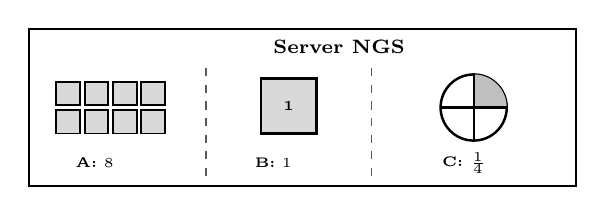
\begin{tikzpicture}[x=1cm, y=1cm, every node/.style={font=\tiny, text=black}]
      % Packet icons: 8 packets | 1 packet | 1/4 disk
      \draw[black, line width=0.8pt, fill=white] (0, 0.05) rectangle (6.95, 2.05);
      \node[font=\scriptsize] at (3.475, 1.82) {\textbf{សង្ខេបលទ្ធផល \en{Server NGS}}};

      % A: 8 packets (2x4 mini squares)
      \foreach \r in {0,1}{
        \foreach \c in {0,1,2,3}{
          \draw[black, line width=0.7pt, fill=headgray] (0.35+\c*0.36, 0.72+\r*0.36) rectangle (0.65+\c*0.36, 1.02+\r*0.36);
        }
      }
      \node at (1.03, 0.35) {\textbf{A: $8$ កញ្ចប់}};

      \draw[darkline, dashed] (2.25, 0.18) -- (2.25, 1.55);

      % B: 1 full packet
      \draw[black, line width=1.0pt, fill=headgray] (2.95, 0.72) rectangle (3.65, 1.42);
      \node at (3.30, 1.07) {$\mathbf{1}$};
      \node at (3.30, 0.35) {\textbf{B: $1$ កញ្ចប់}};

      \draw[darkline, dashed] (4.35, 0.18) -- (4.35, 1.55);

      % C: 1/4 disk shaded
      \draw[black, line width=0.9pt, fill=white] (5.65, 1.05) circle (0.42);
      \fill[midgray] (5.65, 1.05) -- (5.65, 1.47) arc (90:0:0.42) -- cycle;
      \draw[black, line width=0.8pt] (5.65, 0.63) -- (5.65, 1.47);
      \draw[black, line width=0.8pt] (5.23, 1.05) -- (6.07, 1.05);
      \node at (5.65, 0.35) {\textbf{C: $\frac{1}{4}$ ថាស}};
    \end{tikzpicture}
  \end{minipage}
\end{tcolorbox}

\vspace{10pt}
\begin{tcolorbox}[enhanced, sharp corners, colback=white, colframe=black, boxrule=0.75pt, boxsep=1pt, top=5pt, bottom=5pt, left=5pt, right=5pt, after skip=10pt]
  \centering\fontsize{7.7pt}{10.8pt}\selectfont
  \textbf{រំលឹកធនាគារហេតុផល៖} \cnum{1} $\frac{a^m}{a^n}=a^{m-n}$ ($a\neq 0$) \en{|} \cnum{2} $a^0=1$ ($a\neq 0$) \en{|} \cnum{3} $a^{-n}=\frac{1}{a^n}$ \& $\frac{1}{a^{-n}}=a^n$ \en{|} \cnum{4} $m-(-n)=m+n$ \& $x=x^1$ \en{|} \cnum{5} ផ្ដុំមេគុណ/គុណ ២.២
\end{tcolorbox}

\begin{tcolorbox}[enhanced, sharp corners, colback=panelgray, colframe=black, boxrule=0.9pt, boxsep=1pt, top=7pt, bottom=7pt, left=7pt, right=7pt]
  \raggedright\fontsize{7.95pt}{11.8pt}\selectfont
  \textbf{ការវាយតម្លៃដៃគូ ៣ តួនាទី (\en{Pause-Ask \& Pause-Review Sign-Off})៖}\\[4pt]
  \chkbox~គ្រប់ \en{Pause-Ask!} ត្រូវបានពិភាក្សា \quad \chkbox~មិនភ្លេចដែនកំណត់ $x,y\neq 0$ \quad \chkbox~បិទ \en{E1} ($8$, $1$, $\frac{1}{4}$) ត្រឹមត្រូវ\\[5pt]
  \textbf{ចំណុចដែលក្រុមយើងប្រយ័ត្នបានល្អជាងគេ៖} $\underline{\hspace{11.2cm}}$\\[5pt]
  \textbf{ហត្ថលេខាត្រួតពិនិត្យ (តួនាទី ៣)៖} $\underline{\hspace{4.4cm}}$ \hfill \textbf{ពិន្ទុភាពច្បាស់ក្រុម (១--៥)៖} $\underline{\hspace{1.4cm}}\,\en{/5}$
\end{tcolorbox}

\clearpage

% ============================================================================
% ទំព័រទី ៥៖ កាតវិនិច្ឆ័យរហ័ស E5 Exit Foils A, B, C, D (កាត់ ៤ ប័ណ្ណ + ចម្លើយគ្រូ)
% ============================================================================
\pagebanner{សម្ភារៈទី ៥៖ កាតវិនិច្ឆ័យរហ័ស \enbf{E5 Exit Foils (A, B, C, D) --} កាត់ ៤ ប័ណ្ណ \scissors}{ទំព័រ ៥/៦ \en{-- E5 Diagnostic}}

{\fontsize{8.1pt}{11.4pt}\selectfont
\textbf{វិធីប្រើក្នុងថ្នាក់ (\en{E5} ៤ នាទីចុងក្រោយ)៖} កាត់ចែកជា ៤ កាត ($A, B, C, D$) $\to$ សិស្សគូស \textbf{ពិត (\ding{51})} ឬ \textbf{ខុស/អន្ទាក់ (\ding{55})}, គូសធនាគារហេតុផល \cnum{1}--\cnum{5} ដែលពាក់ព័ន្ធ និងកែតម្រូវចម្លើយខុស! \textit{(ការរំលេចកំហុសក្រោយ \en{E4} តាម \en{Ngu et al., 2025} និង \en{Pramasdyahsari et al., 2024})}}

\vspace{5pt}

% ម៉ាក្រូសំណុំប្រអប់ធនាគារហេតុផល
\newcommand{\warrantChecks}{%
  \textbf{ហេតុផលពាក់ព័ន្ធ៖} \chkbox~\cnum{1} \quad \chkbox~\cnum{2} \quad \chkbox~\cnum{3} \quad \chkbox~\cnum{4} \quad \chkbox~\cnum{5}%
}

% --- ជួរទី ១៖ កាត A & កាត B ---
\noindent
\begin{tcolorbox}[
  enhanced, sharp corners, colback=white, colframe=white,
  borderline={1.0pt}{0pt}{black, dashed},
  width=9.25cm, equal height group=powfoilrow1, nobeforeafter,
  boxsep=1pt, top=6pt, bottom=6pt, left=6pt, right=6pt
]
  \noindent\colorbox{black}{\textcolor{white}{\Large\textbf{\en{ A }}}}\hspace{0.22cm}{\fontsize{8.6pt}{11.5pt}\selectfont\textbf{កាត \en{A} ៖ អន្ទាក់ចែកគោល និងចែកនិទស្សន្ត}}\par\vspace{4pt}
  {\fontsize{7.4pt}{10pt}\selectfont ឈ្មោះ/ក្រុម៖ $\underline{\hspace{3.8cm}}$ \hfill លេខតុ៖ $\underline{\hspace{1.1cm}}$}\par\vspace{5pt}
  \begin{tcolorbox}[enhanced, sharp corners, colback=panelgray, colframe=black, boxrule=0.85pt, boxsep=1pt, top=9pt, bottom=9pt, left=5pt, right=5pt]
    \centering\fontsize{10.5pt}{14pt}\selectfont
    $\dfrac{6^8}{6^2} = 1^4 = 1$
  \end{tcolorbox}
  \par\vspace{6pt}\raggedright\fontsize{7.95pt}{11.8pt}\selectfont
  \textbf{១. ការវិនិច្ឆ័យ៖} \quad \chkbox~ពិត (\ding{51}) \qquad \chkbox~ខុស/អន្ទាក់ (\ding{55})\\[4pt]
  \textbf{២.} \warrantChecks\\[4pt]
  \textbf{៣. បើខុស ចូរសរសេរចម្លើយត្រឹមត្រូវ និងពន្យល់៖}\\[4pt]
  ចម្លើយត្រូវ៖ $\underline{\hspace{6.2cm}}$\\[4pt]
  មូលហេតុ៖ $\underline{\hspace{6.4cm}}$\\[5pt]
  $\underline{\hspace{8.2cm}}$
\end{tcolorbox}%
\hfill
\begin{tcolorbox}[
  enhanced, sharp corners, colback=white, colframe=white,
  borderline={1.0pt}{0pt}{black, dashed},
  width=9.25cm, equal height group=powfoilrow1, nobeforeafter,
  boxsep=1pt, top=6pt, bottom=6pt, left=6pt, right=6pt
]
  \noindent\colorbox{black}{\textcolor{white}{\Large\textbf{\en{ B }}}}\hspace{0.22cm}{\fontsize{8.6pt}{11.5pt}\selectfont\textbf{កាត \en{B} ៖ អន្ទាក់ដកនិទស្សន្តអវិជ្ជមាន ($a\neq 0$)}}\par\vspace{4pt}
  {\fontsize{7.4pt}{10pt}\selectfont ឈ្មោះ/ក្រុម៖ $\underline{\hspace{3.8cm}}$ \hfill លេខតុ៖ $\underline{\hspace{1.1cm}}$}\par\vspace{5pt}
  \begin{tcolorbox}[enhanced, sharp corners, colback=panelgray, colframe=black, boxrule=0.85pt, boxsep=1pt, top=9pt, bottom=9pt, left=5pt, right=5pt]
    \centering\fontsize{10.5pt}{14pt}\selectfont
    $\dfrac{a^5}{a^{-3}} = a^2 \quad (a\neq 0)$
  \end{tcolorbox}
  \par\vspace{6pt}\raggedright\fontsize{7.95pt}{11.8pt}\selectfont
  \textbf{១. ការវិនិច្ឆ័យ៖} \quad \chkbox~ពិត (\ding{51}) \qquad \chkbox~ខុស/អន្ទាក់ (\ding{55})\\[4pt]
  \textbf{២.} \warrantChecks\\[4pt]
  \textbf{៣. បើខុស ចូរសរសេរចម្លើយត្រឹមត្រូវ និងពន្យល់៖}\\[4pt]
  ចម្លើយត្រូវ៖ $\underline{\hspace{6.2cm}}$\\[4pt]
  មូលហេតុ៖ $\underline{\hspace{6.4cm}}$\\[5pt]
  $\underline{\hspace{8.2cm}}$
\end{tcolorbox}

\vspace{8pt}
\noindent\scissors\ \dotfill\ \textbf{កាត់តាមស្នាមចុចចែកជា ៤ កាត (\en{Cut Along Dashed Lines})} \dotfill\ \scissors
\vspace{8pt}

% --- ជួរទី ២៖ កាត C & កាត D ---
\noindent
\begin{tcolorbox}[
  enhanced, sharp corners, colback=white, colframe=white,
  borderline={1.0pt}{0pt}{black, dashed},
  width=9.25cm, equal height group=powfoilrow2, nobeforeafter,
  boxsep=1pt, top=6pt, bottom=6pt, left=6pt, right=6pt
]
  \noindent\colorbox{black}{\textcolor{white}{\Large\textbf{\en{ C }}}}\hspace{0.22cm}{\fontsize{8.6pt}{11.5pt}\selectfont\textbf{កាត \en{C} ៖ កន្សោមពហុអថេរ និងនិទស្សន្ត $0$ ($a,b\neq 0$)}}\par\vspace{4pt}
  {\fontsize{7.4pt}{10pt}\selectfont ឈ្មោះ/ក្រុម៖ $\underline{\hspace{3.8cm}}$ \hfill លេខតុ៖ $\underline{\hspace{1.1cm}}$}\par\vspace{5pt}
  \begin{tcolorbox}[enhanced, sharp corners, colback=panelgray, colframe=black, boxrule=0.85pt, boxsep=1pt, top=9pt, bottom=9pt, left=5pt, right=5pt]
    \centering\fontsize{10.2pt}{14pt}\selectfont
    $\dfrac{-8a^3 b^{-2}}{2a^3 b^{-5}} = -4b^3 \quad (a,b\neq 0)$
  \end{tcolorbox}
  \par\vspace{6pt}\raggedright\fontsize{7.95pt}{11.8pt}\selectfont
  \textbf{១. ការវិនិច្ឆ័យ៖} \quad \chkbox~ពិត (\ding{51}) \qquad \chkbox~ខុស/អន្ទាក់ (\ding{55})\\[4pt]
  \textbf{២.} \warrantChecks\\[4pt]
  \textbf{៣. បង្ហាញជំហានផ្ទៀងខ្លី ឬកែតម្រូវ៖}\\[4pt]
  ផ្ទៀង/កែ៖ $\underline{\hspace{6.5cm}}$\\[4pt]
  មូលហេតុ៖ $\underline{\hspace{6.4cm}}$\\[5pt]
  $\underline{\hspace{8.2cm}}$
\end{tcolorbox}%
\hfill
\begin{tcolorbox}[
  enhanced, sharp corners, colback=white, colframe=white,
  borderline={1.0pt}{0pt}{black, dashed},
  width=9.25cm, equal height group=powfoilrow2, nobeforeafter,
  boxsep=1pt, top=6pt, bottom=6pt, left=6pt, right=6pt
]
  \noindent\colorbox{black}{\textcolor{white}{\Large\textbf{\en{ D }}}}\hspace{0.22cm}{\fontsize{8.6pt}{11.5pt}\selectfont\textbf{កាត \en{D} ៖ អន្ទាក់និទស្សន្តសូន្យ ($a,b\neq 0$)}}\par\vspace{4pt}
  {\fontsize{7.4pt}{10pt}\selectfont ឈ្មោះ/ក្រុម៖ $\underline{\hspace{3.8cm}}$ \hfill លេខតុ៖ $\underline{\hspace{1.1cm}}$}\par\vspace{5pt}
  \begin{tcolorbox}[enhanced, sharp corners, colback=panelgray, colframe=black, boxrule=0.85pt, boxsep=1pt, top=9pt, bottom=9pt, left=5pt, right=5pt]
    \centering\fontsize{10.2pt}{14pt}\selectfont
    $\left(\dfrac{-7a^4}{b^2}\right)^0 = 0 \quad (a,b\neq 0)$
  \end{tcolorbox}
  \par\vspace{6pt}\raggedright\fontsize{7.95pt}{11.8pt}\selectfont
  \textbf{១. ការវិនិច្ឆ័យ៖} \quad \chkbox~ពិត (\ding{51}) \qquad \chkbox~ខុស/អន្ទាក់ (\ding{55})\\[4pt]
  \textbf{២.} \warrantChecks\\[4pt]
  \textbf{៣. បើខុស ចូរសរសេរចម្លើយត្រឹមត្រូវ និងពន្យល់៖}\\[4pt]
  ចម្លើយត្រូវ៖ $\underline{\hspace{6.2cm}}$\\[4pt]
  មូលហេតុ៖ $\underline{\hspace{6.4cm}}$\\[5pt]
  $\underline{\hspace{8.2cm}}$
\end{tcolorbox}

\vspace{9pt}
\noindent\scissors\ \dotfill\ \textbf{កាត់ទុកសម្រាប់គ្រូ (\en{Teacher Answer Key \& Remediation})} \dotfill\ \scissors
\vspace{7pt}

\begin{tcolorbox}[
  enhanced, sharp corners, colback=panelgray, colframe=black,
  boxrule=1.0pt, boxsep=1pt, top=5pt, bottom=5pt, left=5pt, right=5pt
]
  \fontsize{7.85pt}{11.2pt}\selectfont
  \renewcommand{\arraystretch}{1.24}
  \begin{tabular}{|L{4.25cm}|L{4.25cm}|L{4.25cm}|L{4.25cm}|}
    \hline
    \cellcolor{headgray}\textbf{កាត \en{A} ៖ ខុស (\ding{55}) \en{|} \cnum{1}} &
    \cellcolor{headgray}\textbf{កាត \en{B} ៖ ខុស (\ding{55}) \en{|} \cnum{1}, \cnum{4}} &
    \cellcolor{headgray}\textbf{កាត \en{C} ៖ ពិត (\ding{51}) \en{|} \cnum{1}\cnum{2}\cnum{4}\cnum{5}} &
    \cellcolor{headgray}\textbf{កាត \en{D} ៖ ខុស (\ding{55}) \en{|} \cnum{2}} \\ \hline
    \textbf{ត្រូវ៖ $6^{8-2} = 6^6$}។\newline សិស្សច្រឡំចែកគោល ($6\div 6=1$) និងចែកនិទស្សន្ត ($8\div 2=4$) ដូច \en{Ulusoy (2019)}! &
    \textbf{ត្រូវ៖ $a^{5-(-3)} = a^8$}។\newline សិស្សភ្លេចសញ្ញាដកពីរជាន់ ($5-3=2$); ផ្ទៀងតាម $\frac{a^5}{a^{-3}}=a^5\cdot a^3=a^8$ (\cnum{3}, \cnum{5})! &
    \textbf{ពិត!} $\frac{-8}{2} a^{3-3} b^{-2-(-5)}$\newline $= -4 a^0 b^3 = -4(1)b^3 = -4b^3$! \newline \textit{(តេស្ត $a^0=1$ និង $-2+5=+3$)} &
    \textbf{ត្រូវ៖ $= 1$}។\newline កន្សោមក្នុងវង់ក្រចកខុសពី $0$ ($\neq 0$) លើកជាស្វ័យគុណ $0$ ស្មើ $\mathbf{1}$ មិនមែន $0$ ទេ! \\[4pt] \hline
  \end{tabular}
\end{tcolorbox}

\vspace{6pt}
\begin{tcolorbox}[enhanced, sharp corners, colback=white, colframe=black, boxrule=0.8pt, boxsep=1pt, top=5pt, bottom=5pt, left=6pt, right=6pt]
  \centering\fontsize{7.7pt}{11.2pt}\selectfont
  \textbf{គន្លឹះកែលម្អភ្លាមៗ (គ្រូបង្ហាញលើក្ដារខៀន)៖} បើសិស្សលើស $20\%$ ខុសកាត $B$ ឱ្យសិស្សគូសរង្វង់ជុំវិញ $(-3)$ និងសរសេរ $5-(\mathbf{-3}) = 5+3$ មុនដកជានិច្ច; បើខុស $D$ រំលឹកជណ្ដើរ $a^1 \div a = a^0 = 1$!
\end{tcolorbox}

\clearpage

% ============================================================================
% ទំព័រទី ៦៖ ប័ណ្ណកិច្ចការផ្ទះ ជំហានទី ៥ — ៤ ប័ណ្ណក្នុង ១ ទំព័រ A4 (#7 គ, ឃ, ច + អានមុន ៤.១-៤.២)
% ============================================================================
\pagebanner{សម្ភារៈទី ៦៖ ប័ណ្ណកិច្ចការផ្ទះ \enbf{--} ៤ ប័ណ្ណ \enbf{A4 (}ទំ\enbf{.}២៥ លំហាត់ ៧ គ\enbf{,} ឃ\enbf{,} ច\enbf{)}}{ទំព័រ ៦/៦ \en{--} កាត់ ៤ ប័ណ្ណ \scissors}

% ប្រយ័ត្ន៖ ប្រើ {#1} កុំឱ្យជាប់លេខឡាតាំងក្រោយ #1!
\newcommand{\hwslipFourPOW}[1]{%
\begin{tcolorbox}[
  enhanced, sharp corners, colback=white, colframe=white,
  borderline={0.95pt}{0pt}{black, dashed},
  width=9.25cm, equal height group=hwquadPOW, nobeforeafter,
  boxsep=1pt, top=6pt, bottom=6pt, left=5.5pt, right=5.5pt
]
  \begin{tcolorbox}[
    enhanced, sharp corners, colback=headgray, colframe=black,
    boxrule=0.75pt, boxsep=1pt, top=4pt, bottom=4pt, left=4.5pt, right=4.5pt, after skip=6pt
  ]
    \fontsize{7.55pt}{11.0pt}\selectfont
    \textbf{\scissors\ កិច្ចការផ្ទះ ({#1}) \en{|} ២.៣ វិធីចែកស្វ័យគុណ} \hfill \textbf{ចន្ទ ១៦/១១/២០២៦}\\[3pt]
    ឈ្មោះ៖ $\underline{\hspace{3.8cm}}$ \hspace{0.2cm} ថ្នាក់៖ $\underline{\hspace{1.1cm}}$
  \end{tcolorbox}

  \raggedright\fontsize{7.7pt}{11.4pt}\selectfont
  \textbf{លំហាត់ទី ៧ (សៀវភៅទំព័រ ២៥ \en{--} អក្សរ គ, ឃ, ច)៖} ចូរសម្រួលកន្សោមខាងក្រោម \textit{(កំណត់ $a\neq 0,\; b\neq 0,\; x\neq 0$)} និងចុះសំអាង \cnum{1}--\cnum{5} ក្នុងសៀវភៅកិច្ចការផ្ទះ៖\\[6pt]

  \begin{tcolorbox}[enhanced, sharp corners, colback=panelgray, colframe=black, boxrule=0.65pt, boxsep=1pt, top=5.5pt, bottom=5.5pt, left=5pt, right=5pt, after skip=6pt]
    \fontsize{8.35pt}{13.4pt}\selectfont
    \textbf{ក (៧.គ)៖}\; $\dfrac{\left(\frac{3}{2}a^2 b^3\right)(2a^{-3}b^4)}{6a^{-2}b^4} = \underline{\hspace{1.55cm}}$ \hfill [\blankcnum] \\[7pt]
    \textbf{ខ (៧.ឃ)៖}\; $\dfrac{(32a^2 x^8)(-5a^4 x^3)}{5ax(-2a^2 x^2)(-4a^3 x)} = \underline{\hspace{1.20cm}}$ \hfill [\blankcnum] \\[7pt]
    \textbf{គ (៧.ច)៖}\; $\dfrac{\left(\frac{3}{2}a^2 b^3\right)^0 (2a^{-3}b^5)}{6a^{-2}b^4} = \underline{\hspace{1.55cm}}$ \hfill [\blankcnum]
  \end{tcolorbox}

  {\fontsize{7.2pt}{10.5pt}\selectfont
  \textbf{គន្លឹះប្រយ័ត្ន៖} (១) ក្នុង \textbf{៧.ឃ} ផ្ដុំមេគុណលើ-ក្រោម និងគិត $x=x^1$; (២) ក្នុង \textbf{៧.ច} មាន $\left(\frac{3}{2}a^2b^3\right)^0 = 1$ (\cnum{2}) និងនិទស្សន្តអវិជ្ជមាន $a^{-1}=\frac{1}{a}$ (\cnum{3})។\\[5pt]}

  \begin{tcolorbox}[enhanced, sharp corners, colback=white, colframe=black, boxrule=0.7pt, boxsep=1pt, top=4.5pt, bottom=4.5pt, left=5pt, right=5pt, after skip=5.5pt]
    \raggedright\fontsize{7.4pt}{10.8pt}\selectfont
    \textbf{អានមេរៀនបន្ទាប់ទុកជាមុន៖} ៤. លក្ខណៈនៃស្វ័យគុណ (\textbf{៤.១--៤.២, ទំព័រ ១៧--១៨})។
  \end{tcolorbox}

  \begin{tcolorbox}[enhanced, sharp corners, colback=panelgray, colframe=black, boxrule=0.65pt, boxsep=1pt, top=4pt, bottom=4pt, left=4pt, right=4pt]
    \fontsize{6.65pt}{9.8pt}\selectfont
    \textbf{ផ្ទៀង៖} \chkbox~សរសេរ $a,b,x\neq 0$ \en{|} \chkbox~គិត $x=x^1$ \& $(\dots)^0=1$ \en{|} \chkbox~សំអាង \cnum{1}--\cnum{5}
  \end{tcolorbox}
\end{tcolorbox}%
}

\vspace{6pt}
\noindent
\hwslipFourPOW{ប័ណ្ណទី ១}\hfill\hwslipFourPOW{ប័ណ្ណទី ២}

\vspace{14pt}
\noindent\scissors\ \dotfill\ \textbf{កាត់តាមស្នាមចុចចែកជា ៤ ប័ណ្ណ (\en{Cut Along Dashed Lines})} \dotfill\ \scissors
\vspace{14pt}

\noindent
\hwslipFourPOW{ប័ណ្ណទី ៣}\hfill\hwslipFourPOW{ប័ណ្ណទី ៤}

\end{document}
